\documentclass[a4paper,12pt,oneside]{book}

\usepackage{times} % Times new roman font asked in the guideline
%%%%%%%%%%%%%%% Maths symbols %%%%%%%%%%%%%%
\usepackage{amsfonts}
\usepackage{amsmath}
\usepackage{amsthm}
\usepackage{amssymb}
%\usepackage{siunitx}
%%%%%%%%%%%%%%%%%%%% Figures, tables and captions %%%%%%%%
\usepackage{graphicx}
%\usepackage{lscape}
\usepackage{caption} % Changes font of captions by putting [font=sf] before {caption} if required.
%\usepackage{dpfloat} % Ability to place figure on even or odd page using \begin{leftfullpage}
% \usepackage{longtable}
\usepackage{booktabs}
\usepackage{longtable} %for list of acronyms
\usepackage{threeparttable}
\usepackage{subcaption}
\graphicspath{{Figures/}}
%%%%%%%%%%%%%%%%%%%%%% Track review changes %%%%%%%%%%%%%%%
%\usepackage{xcolor}
%\newcommand{\RV}[1]{\textcolor{violet}{#1}}

%%%%%%%%%%%%%%%%%% Numbering lines in verbatim %%%%%%%%%%%%
%\usepackage{fancyvrb}
%%%%%%%%%%%%%%%%%%%%%%%% Appendices %%%%%%%%%%%%%%%%%%%
%\usepackage{appendix}
%%%%%%%%%%%%%%%%%%%%%%%%%% Navigation %%%%%%%%%%%%%%%%%%%
% \usepackage[hidelinks,colorlinks,allcolors=blue]{hyperref} %soft-copy with color hyperlinks
\usepackage[hidelinks]{hyperref} %hard-copy no color hyperlinks

\renewcommand{\sectionautorefname}{Section}	%captitalize first s in Section while using autoref
\renewcommand{\subsectionautorefname}{Subsection}
\renewcommand{\chapterautorefname}{Chapter}
\renewcommand{\itemautorefname}{Item}
\usepackage{bookmark}	%to use startatroot feature
\newcommand*{\fullref}[1]{\hyperref[{#1}]{\autoref*{#1} \nameref*{#1}}} %navigating titles along with numbers

%%%%%%%%%%%%%%%%%% OPTIONAL %%%%%%%%%%%%%%%%%%
%%%%%%%%%%%%%%%%%% Bengali font for few texts and Russian for a specific bibitem %%%%%%%%%%%%%%%%%%%
%%%%%%%%%%%%%%%%%% XeLaTeX compiler with this setting
% \usepackage{polyglossia}
% \setmainlanguage{english}
% \setmainfont{Times New Roman} % Times new roman font asked in the guideline
% \setotherlanguages{bengali, russian}
% \newfontfamily \bn[Scale=0.9,Script=Bengali]{Kalpurush.ttf} % if you want to use this font, you need to place the font file in the root directory
% \newfontfamily \cyrillicfont[Script=Cyrillic]{STIX2Text-Regular.otf} % if you want to use this font, you need to place the font file in the root directory
% \usepackage{tipa}
%%%%%%%%%%%%%%%% References %%%%%%%%%%%%%%%%%%
\usepackage[dashed=false, backend=biber, style=ieee, natbib=true, maxcitenames=2, mincitenames=1, defernumbers=true]{biblatex}
\usepackage{csquotes}
\bibliography{all_references.bib}
\setcounter{biburlnumpenalty}{7000} %to break DOI having strings of numbers
\usepackage[nospacearound]{extdash} %break already dashed word Otolaryngology in a reference
%%%%%%%%%%%%%% Aesthetic, control of margins, headers, etc. %%%%%%%%%%%%%%%
\usepackage{geometry}
\geometry{
left=1.2in,
top=1.2in,
right=1in,
bottom=1in
}
\setlength{\headheight}{14.49998pt} % fancyhdr need space on top
\usepackage{fancyhdr,layout}
\usepackage{etoolbox}		%to use appto command
%\oddsidemargin 1.6 cm
%\evensidemargin 0.4 cm
\pagestyle{fancy}
\renewcommand{\chaptermark}[1]{\markboth{\MakeUppercase{\chaptername}\ \thechapter.\ #1}{}}		%changing the chaptermark
%\renewcommand{\sectionmark}[1]{\markright{\thesection\ #1}} %not used
\fancypagestyle{main}{%		%pagestyles for mainmatter
\fancyhf{}
% \fancyhead[LE,RO]{\bfseries\thepage}	%page number at HeaderCenter for both even and odd pages % if I make it for two-sided book-like printing
\fancyhead[R]{\bfseries\thepage}	%page number at HeaderCenter for both even and odd pages % If I make it for single-sided printing
%\fancyhead[LO]{\bfseries\rightmark}	%left of odd pages: sectionmark
% \fancyhead[LO]{\bfseries\leftmark}	%left of odd pages: chaptermark % if I make it for two-sided book-like printing
% \fancyhead[L]{\bfseries\leftmark}	%left of odd pages: chaptermark % If I make it for single-sided printing
%\fancyhead[RE]{\bfseries\leftmark} %right of even page: chaptermark %no use in one-side printing
\renewcommand{\headrulewidth}{0pt}	%width of the header rule
\renewcommand{\footrulewidth}{0pt}

}
% \usepackage{titlesec}
% \newcommand{\abstractfont}{\Large\bfseries} % Adjust as needed
% \newcommand{\acknowledgmentfont}{\Large\bfseries} % Adjust as needed
% \newcommand{\abstractmarginskip}{16pt}

%\addtolength{\headheight}{14.5pt}
\setlength{\footskip}{.3in}
\renewcommand{\footruleskip}{0pt}
\fancypagestyle{main}{% page style for mainmatter
  \fancyhf{} % clear header and footer
  \fancyfoot[C]{\normalfont\thepage} % page number at FooterCenter for both even and odd pages
  \renewcommand{\headrulewidth}{0pt} % width of the header rule
  \renewcommand{\footrulewidth}{0pt} % no footer rule
}

\fancypagestyle{plain}{% redefining plain page style for first few pages
  \fancyhf{} % clear header and footer
  \fancyfoot[C]{\normalfont\thepage} % page number at FooterCenter
  \renewcommand{\headrulewidth}{0pt}
  \renewcommand{\footrulewidth}{0pt}
}

\pagestyle{main} % Set the default page style
% \fancypagestyle{plain}{%		%redefining plain page style for first few pages
% \fancyhf{}
% % \fancyhead[LE,RO]{\bfseries\thepage} % if I make it for two-sided book-like printing
% \fancyhead[R]{\bfseries\thepage} % If I make it for single-sided printing
% \renewcommand{\headrulewidth}{0pt}
% }
\appto\frontmatter{\pagestyle{plain}}
\appto\mainmatter{\pagestyle{main}}
%%%%%%%%%%%%%%%%%%%%%%%%%%% Others %%%%%%%%%%%%%%%%%%%%%
\usepackage{enumerate}
\usepackage{array}	%to use arraybackslash in table
\usepackage{calc}		%to add two length variable
%\usepackage{anyfontsize}

%%%%%%%%%%%%%%%%%%%%%% Control of chapter/section headings according to the guidelines %%%%%%%%%%%%%%%%%%%%%
\usepackage[explicit]{titlesec}

%change the chapter number to Roman only after CHAPTER. But the below first command also changes the chapter number everywhere including section, figures, etc. numbering. So, section, figure, etc numbers are kept at arabic again
\renewcommand{\thechapter}{\Roman{chapter}}
\renewcommand{\thesection}{\arabic{chapter}.\arabic{section}}
\renewcommand{\thefigure}{\arabic{chapter}.\arabic{figure}}
\renewcommand{\thetable}{\arabic{chapter}.\arabic{table}}
\renewcommand{\theequation}{\arabic{chapter}.\arabic{equation}}

\titleformat{\chapter}[display]{\normalfont\bfseries\filcenter}{\MakeUppercase\chaptertitlename\  \thechapter}{24pt}{{#1}}	%CHAPTER with a space
\titleformat{\chapter}[display]{\fontsize{14}{16.8}\selectfont\bfseries\filcenter}{\MakeUppercase\chaptertitlename\ \thechapter}{14pt}{{#1}} % large font size rather than what mentioned in guideline
%\titlespacing*{\chapter}{0pt}{0pt}{24pt}  %KUET guideline. The command controls vertical margins on title; {left}{before-sep}{after-sep}
\titlespacing*{\chapter} {0pt}{-40pt}{40pt} % slightly changed to look better

\titleformat{\section}{\normalfont\bfseries}{\thesection}{0.65em}{#1}
%\titlespacing*{\section}{0pt}{24pt}{12pt} 
\titlespacing*{\section} {0pt}{3.5ex plus 1ex minus .2ex}{1.5ex plus .2ex}	

\titleformat{\subsection}{\normalfont\bfseries}{\thesubsection}{.65em}{#1}
%\titlespacing*{\subsection}{0pt}{20pt}{10pt}
\titlespacing*{\subsection} {0pt}{3.5ex plus 1ex minus .2ex}{1.5ex plus .2ex}

\titleformat{\subsubsection}{\normalfont\bfseries}{\thesubsubsection}{0.65em}{#1}
\titlespacing*{\subsubsection}{0pt}{3.25ex plus 1ex minus .2ex}{.5ex plus .2ex}

%standard spacings from titlesec doc
%\titlespacing*{\chapter} {0pt}{50pt}{40pt}
%\titlespacing*{\section} {0pt}{3.5ex plus 1ex minus .2ex}{2.3ex plus .2ex}
%\titlespacing*{\subsection} {0pt}{3.25ex plus 1ex minus .2ex}{1.5ex plus .2ex}
%\titlespacing*{\subsubsection}{0pt}{3.25ex plus 1ex minus .2ex}{1.5ex plus .2ex}
%\titlespacing*{\paragraph} {0pt}{3.25ex plus 1ex minus .2ex}{1em}
%\titlespacing*{\subparagraph} {\parindent}{3.25ex plus 1ex minus .2ex}{1em}

%%%%%%%%%%%%%%%%%%%%%%% Line Spacing %%%%%%%%%%%%%%%%%%
% spacing 1.5
%\linespread{1.5} 
%\renewcommand{\baselinestretch}{1.5}		%controlling linespacing useing baselinestretch changing, similar to the linespread command. It changes the spacing for everything in the document, including footnotes and tables
%\newcommand{\spacingR}[1]{\linespread{#1}\selectfont}		%different linespacing within the document if linespread is used
\usepackage{setspace}
%\captionsetup{font={stretch=1.5}}	%to address: setspace doesn't change the figure/table captions
\setstretch{1.5}	%onehalfspacing of LaTeX doesn't match with MS Word's 1.5 spacing, so tuned this value. Probably MS Word's 1.5 spacing is equivalent to (slightly less than) doublespaing in LaTeX
%\onehalfspacing
%%%%%%%%%%%%% control the style of toc, lof, lot %%%%%%%%%%%%%%%%
\usepackage{tocloft}
%making toc centered
\renewcommand{\cfttoctitlefont}{\hfill\fontsize{16}{19.2}\selectfont\bfseries}
\renewcommand{\cftaftertoctitle}{\hfill} 
\setlength{\cftbeforetoctitleskip}{-15pt} % Adjust this value as needed
\setlength{\cftaftertoctitleskip}{50pt}
\addtocontents{toc}{~\hfill\textbf{PAGE}\par}	%to pring the word "Page" above the page numbers
%making lot centered
\renewcommand{\cftlottitlefont}{\hfill\fontsize{16}{19.2}\selectfont\bfseries\MakeLowercase{}}
\renewcommand{\cftafterlottitle}{\hfill} 
%making lof centered
\renewcommand{\cftloftitlefont}{\hfill\fontsize{16}{19.2}\selectfont\bfseries\MakeLowercase{}}
\renewcommand{\cftafterloftitle}{\hfill} 

\setlength{\cftbeforelottitleskip}{-15pt} % Space above LOT title
\setlength{\cftafterlottitleskip}{50pt} % Space below LOT title
\setlength{\cftbeforeloftitleskip}{-15pt} % Space above LOF title
\setlength{\cftafterloftitleskip}{50pt} % Space below LOF title

\renewcommand{\cftpnumalign}{c} %center align the page numbers
\cftsetpnumwidth{1.9em}	%so that the alighment looks good with the title "Page"
%write CHAPTER in front of chapter
\renewcommand{\cftchapfont}{}		%removing boldface
\renewcommand{\cftchappagefont}{} 	%removing boldface from page numbers
\renewcommand{\cftchappresnum}{\bfseries CHAPTER } 
\renewcommand{\cftchapaftersnum}{\quad}	%some space after chapter number
\newlength{\mylen} % a "scratch" length
\settowidth{\mylen}{\bfseries\cftchappresnum\cftchapaftersnum} % extra space
\addtolength{\cftchapnumwidth}{\mylen} % add the extra space

\cftsetindents{section}{\cftchapnumwidth}{\cftsecnumwidth} %pushing extra indent to put right below chapter title. Extra indents equal already calculated extra space (i.e., cftchapnumwidth) created by "CHAPTER " word. Section numwidth default value as cftsecnumwidth kept unaltered.
\newlength{\mysecondlen}
\setlength{\mysecondlen}{\cftchapnumwidth+\cftsecnumwidth} %subsection indent=chapter numwidth plus section numwidth
\cftsetindents{subsection}{\mysecondlen}{\cftsubsecnumwidth} %indentation for subsection just like section

% as per guideline, no dots linking to page number
\renewcommand{\cftsecdotsep}{\cftnodots} %section
\renewcommand{\cftsubsecdotsep}{\cftnodots} %subsection
\renewcommand{\cftfigdotsep}{\cftnodots} %figure; looks weird for multi-line captions
\renewcommand{\cfttabdotsep}{\cftnodots} %table; looks weird for multi-line captions

%formatting frontmatter contents
\renewcommand{\cftpartfont}{}		%removing boldface
\renewcommand{\cftpartpagefont}{\normalfont} 	%removing boldface from page numbers and giving normalfont
\setlength{\cftbeforepartskip}{1.5mm} %reducing vertical space in front matters of contents
\cftsetindents{part}{3em}{\cftpartnumwidth} %extra indentation as per guideline

%%%%%%%%%%%%%%%%%%%%%% Paragraph Indentation %%%%%%%%%%%%%%%
\usepackage{parskip}	%to have a vartical space instead of indentation in paragraph... as per guideline. It has a slight clash with the tocloft package; suggested to declare after toclof
\usepackage[absolute,overlay]{textpos}
\usepackage{pgfgantt}

 % the packages and their settings in a separate file
%%%%%%%%%%%%%%%%%%%% Some new custom commands %%%%%%%%%%%%%%%%%
\newcommand{\blanklineR}{\hfill \\} %to have blanklines
\newcommand{\HeadingR}[1]{%	font size 14 and boldface for headings
%\fontsize{14}{21}{% baselinestrech 1.5, so 14*1.5=21
%\selectfont
% \DeclareCaptionFont{customfont}{\fontsize{11}{13}\selectfont}
% \captionsetup{font=customfont}

{\fontsize{16}{19.2}\selectfont			%large equals 14pt when the document is 12pt
\bfseries{#1}}
\vspace{35pt}
}
\newcommand{\titleR}{Depth Map Generation Using Monocular Depth Estimation of Deep Learning}		%title strored as command so that I can adapt easily if any change occurs

%%%%%%%%%%%%%%%%% PDF meta-data %%%%%%%%%%%%%%%%%%%%%%%%
\hypersetup{%
pdfauthor={Your name},
pdftitle=\titleR,
pdfsubject={BSc Eng. Thesis},
pdfkeywords={}
}
%%%%%%%%%%%%%%%%%%%%%%%%%%%%%%%%%%%%%%%%%%%%%%%%%%%%%%%%%%%%%%%%%%%%%%%%%%%%%%%%%%%%%%%%%%%%
%%%%%%%%%%%%%%%%%%%%%%%%%%%% DOCUMENT STARTS %%%%%%%%%%%%%%%%%%%%%%%%%%%%%%%%%%%%%%%%%%%%%%%%%%%
%%%%%%%%%%%%%%%%%%%%%%%%%%%%%%%%%%%%%%%%%%%%%%%%%%%%%%%%%%%%%%%%%%%%%%%%%%%%%%%%%%%%%%%%%%%%
\begin{document}
\frontmatter
%%%%%%%%%%%%%%%%%%% Title Page %%%%%%%%%%%%%%%%%%%%%
% \begin{textblock*}{\paperwidth}(1.2in,0.5in)
%   {\fontsize{12}{18}\selectfont Project/Thesis No. :}
% \end{textblock*}

\begin{titlepage}
    \centering
    \begin{flushleft}
        \textbf{\fontsize{14}{21}\selectfont Thesis No: CSER-24-58}
    \end{flushleft}
    \vspace{0pt}
    
    \textsc{\textbf{\fontsize{18}{27}\selectfont Depth Map Generation Using Monocular Depth Estimation of Deep Learning\\}}
    
    \vspace{36pt}
    
    {\fontsize{14}{21}\selectfont By\\}
    \vspace{54pt}
    
    \textbf{\fontsize{14}{21}\selectfont Dabbrata Das\\}
    {\fontsize{14}{21}\selectfont Roll: 1807109\\}

    \vspace{78pt}

    
\includegraphics[width=1in,height=1.2in]{Figures/logo.png}\\

    \vspace{104pt}
    
    \textbf{\fontsize{12}{18}\selectfont Department of Computer Science and Engineering\\
    Khulna University of Engineering \& Technology\\
    Khulna 9203, Bangladesh\\
    February, 2024\\
    }
        
\end{titlepage}
\newpage
% \addtocounter{page}{1}	%otherwise, this page number becomes (i)
\phantomsection \label{declar}
\addcontentsline{toc}{part}{Title Page}
\begin{center}
%\begin{onehalfspacing}
%\linespread{1.3}
\textbf{\fontsize{18}{27}\selectfont Depth Map Generation Using Monocular Depth Estimation of Deep Learning\\}
\blanklineR\blanklineR\blanklineR
By\\
\blanklineR\blanklineR
\textbf{Dabbrata Das}\\
\text{Roll: 1807109}
\blanklineR\blanklineR\blanklineR\blanklineR
A thesis submitted in partial fulfillment of the requirements for the degree of \\
“Bachelor of Science in Computer Science and Engineering”\\
\blanklineR\blanklineR
\begin{flushleft}
        {\fontsize{12}{18} \textbf{Supervisor:}}
        \begin{tabular}{p{12cm} p{4cm}}
                \hspace{0.8 in}\textbf{Dr. Pintu Chandra Shill}                &                                \\
                \hspace{0.8 in}Professor                                      & \multicolumn{1}{l}{\rule{1.1in}{\arrayrulewidth}}          \\
                \hspace{0.8 in}Department of Computer Science and Engineering & \multicolumn{1}{l}{\hspace{16pt}Signature} \\
                \hspace{0.8 in}Khulna University of Engineering \& Technology & \vspace{36pt}
            \end{tabular}
    \end{flushleft}

\blanklineR\blanklineR\blanklineR
Department of Computer Science and Engineering \\
Khulna University of Engineering \& Technology\\
Khulna 9203, Bangladesh\\
\text{February, 2024}
\end{center}

% \newpage
% %%%%%%%%%%%%%%%%% Declaration %%%%%%%%%%%%%%%%%%%%%%%%%%
% % \addtocounter{page}{1}	%otherwise, this page number becomes (i)
% \phantomsection \label{declar}
% \addcontentsline{toc}{part}{Declaration}

% \begin{center}
% \HeadingR{Declaration}\\
% \end{center}
% \blanklineR\blanklineR\blanklineR
% This is to certify that the thesis work entitled \textit{``\titleR"} has been carried out by \textit{Your name} in the Department of \textit{Electrical and Electronic Engineering}, Khulna University of Engineering \& Technology, Khulna, Bangladesh. The above thesis work or any part of this work has not been submitted anywhere for the award of any degree or diploma.\\[2cm]

% \begin{center}
% \begin{tabular}{*2c}
% \parbox{0.49\textwidth}{\centering Signature of Supervisor} & \parbox{0.49\textwidth}{\centering Signature of Candidate}
% \end{tabular}
% \end{center}
% %%%%%%%%%%%%%%%%% Approval %%%%%%%%%%%%%%%%%%%%%%%%%%
% \newpage
% \phantomsection \label{approval}
% \addcontentsline{toc}{part}{Approval}
% \begin{center}
% \HeadingR{Approval}
% \blanklineR
% \end{center}
% This is to certify that the thesis work submitted by \textit{Your name} entitled \textit{``\titleR"} has been approved by the board of examiners for the partial fulfillment of the requirements for the degree of \textit{Master of Science in Engineering (M. Sc. Eng.)} in the Department of \textit{Electrical and Electronic Engineering}, Khulna University of Engineering \& Technology, Khulna, Bangladesh in October 2021.
% \begin{center}
% \textbf{BOARD OF EXAMINERS}
% \vspace{5mm}

% \begin{singlespacing}
% \begin{tabular}{p{1mm}p{0.7\textwidth}>{\centering\arraybackslash}p{0.2\textwidth}}
% 1. & \rule{0.32\textwidth}{\arrayrulewidth}\newline Your supervisor's name\newline Professor\newline Department of Electrical and Electronic Engineering\newline Khulna University of Engineering \& Technology & Chairman (Supervisor)\\[6em]
% 2. & \rule{0.32\textwidth}{\arrayrulewidth}\newline Head of the Department\newline Department of Electrical and Electronic Engineering\newline Khulna University of Engineering \& Technology & Member \\[6em]
% 3. & \rule{0.32\textwidth}{\arrayrulewidth}\newline Internal member's name\newline Professor\newline Department of Electrical and Electronic Engineering\newline Khulna University of Engineering \& Technology & Member \\[7em]
% 4. & \rule{0.32\textwidth}{\arrayrulewidth}\newline Another internal member's name\newline Professor\newline Department of Electrical and Electronic Engineering\newline Khulna University of Engineering \& Technology & Member \\[7em]
% 5. & \rule{0.32\textwidth}{\arrayrulewidth}\newline External member's name\newline Professor\newline Department of Electrical and Electronic Engineering\newline Bangladesh University of Engineering and Technology & Member (External) \\
% \end{tabular}
% \end{singlespacing}
% \end{center}

%%%%%%%%%%%%%%%%%%%% Acknowledgments %%%%%%%%%%%%%%%%%%%%%%%%%
\newpage
\phantomsection \label{ack}
\addcontentsline{toc}{part}{Acknowledgments}

\begin{center}
\HeadingR{Acknowledgements}
\end{center}
We would like to express my deepest gratitude to the Almighty Creator, the source of all knowledge and wisdom, whose divine guidance and blessings have illuminated our path throughout the journey of this thesis. We are immensely thankful for the strength and resilience that faith in the Creator has instilled in us during the challenging phases of this research. Your divine grace has been our constant source of inspiration and motivation, helping us persevere in the face of obstacles. We are also grateful for the unwavering support and encouragement of our family, friends, and mentors who have been instrumental in shaping this thesis. Their belief in us and their prayers have been invaluable.\\\\

\begin{flushright}
\textbf{Authors}
\end{flushright}

   
%%%%%%%%%%%%%%%%%%%% Abstract %%%%%%%%%%%%%%%%%%%%%%%%%
\newpage
\phantomsection \label{abstr}
\addcontentsline{toc}{part}{Abstract}

\begin{center}
\HeadingR{Abstract}
\end{center}
Monocular depth estimation is one of the most important tasks in computer vision and the estimation based on deep learning plays a significant role in various fields
such as autonomous driving, navigation system with tracking, augmented reality, etc. There are some existing solutions of depth estimation which produced blurry, low-resolution and lower accurate depth map with higher cost. In this report, it presents a convolution neural network (CNN) for computing depth map with the help of transfer learning approaches where a single RGB image is given. Here U-Net architecture is followed which basically an encoder-decoder architecture. In encoder section some high performing pretrained models are applied which can extract more accurate features from the image along with augmentation and lead to more accurate result. A very simple decoder is used which decoded required depth map with lower number of parameters and generates more detailed depth map. Besides tuning the loss function increases more accuracy of the depth map. There are different types of datasets and models which are mostly used for the improvement among them NYU-DepthV2 dataset is used to estimate the depth map.
Using the specific dataset with transfer learning approaches, the U-Net architecture will be able to generate a more detailed and more accurate depth map with better resolution.
Finally, the improvements and  the challenges which will arise in monocular depth estimation from a single RGB image will also be highlighted here.

%%%%%%%%%%%%%%%%%%% Contents %%%%%%%%%%%%%%%%
\newpage
\phantomsection \label{cont}
\addcontentsline{toc}{part}{Contents}
\currentpdfbookmark{\contentsname}{toc}
\begin{singlespacing}
\tableofcontents
\end{singlespacing}


%%%%%%%%%%%%%%% Include list of tables (and in table of contents) %%%%%%%%%%%%%%%
\newpage
\phantomsection \label{listoftab}
\addcontentsline{toc}{part}{List of Tables}
\listoftables
\addtocontents{lot}{\textbf{Table No.}\hfill \textbf{Description}\hfill\textbf{Page}\par}	%to pring above the page numbers
% Include list of figures (and in table of contents)
\newpage
\phantomsection \label{listoffig}
\addcontentsline{toc}{part}{List of Figures}
\listoffigures
\addtocontents{lof}{\textbf{Figure No.}\hfill \textbf{Description}\hfill\textbf{Page}\par}	%to pring above the page numbers

%%%%%%%%%%%%%%%%%%%% Acknowledgments %%%%%%%%%%%%%%%%%%%%%%%%%
% \newpage
% \phantomsection \label{abbrv}
% \addcontentsline{toc}{part}{List of Acronyms}

% \begin{center}
% \HeadingR{\MakeUppercase{List of Acronyms}}
% \blanklineR \blanklineR
% \begin{longtable}{l@{\qquad}l}
% KUET & Khulna University of Engineering \& Technology \\
% EEE & Electrical and Electronic Engineering 
% \end{longtable}
% \end{center}

\mainmatter
\bookmarksetup{startatroot} %front and backmatters are defined as part; so the bookmark hierarchy of the below chapters falls below the part, whereas I want them in the same level. This command from bookmark package works like a charm
%%%%%%%%%%%%%%%%%%%%%% Introduction %%%%%%%%%%%%%%%%%%%%%%%%%%%%
\chapter{\textbf{Introduction}}\label{chap:intro}
\section{Introduction}\label{sec:intro}
Monocular depth estimation is one of the most advanced tasks in the field of computer vision. Depth estimation means estimate the depth of the objects or find the relative distance between two objects from an image. And depth map is an image which contains depth information of the image and is generated using depth estimation.There are different kinds of deep learning models like U-Net \cite{unetwotk}, AlexNet \cite{alexnetwork}, ResNet \cite{resnetwork}, etc and functions such as evaluation functions, loss functions, etc. and datasets such as DIODE, NYU Depth V2, KITTI, etc. used as the basic tools for the implementation of the project.In this report, Convolution Neural Network is used for the task of depth estimation followed by U-Net architecture where U-Net architecture is basically an endcoder-decoder based architecture.Besides some high performing pretrained models are used with this architecture as encoder part which provide high quality depth map with better accuracy than normal encoder.Nyu Depth V2 data is used which is basically consisted with indoor RGB images with Ground Truth depth map provides more accurate result after training. Resnet50, Densenet169, VGG19 and Inception Resnet V2 are high performing pre-trained networks that are originally designed for image classification as the deep features encoder.
\section{Background}\label{sec:backg}
Obtaining a depth map accurately is too much hard task which requires heavy costs and a lot of resources with times. Besides it is also possible to calculate the accurate depth map through sensors like LiDaR. But it is too much costly and time-consuming. So monocular depth
estimation is highly necessary to meet up the problem where a single RGB image is needed as input and provide a depth map with good accuracy through well-trained depth estimation model.

\section{Objectives}
The main goal is to generate an accurate depth map with higher visual quality using monocular depth estimation approach. Besides, the other objectives are:

\begin{singlespacing}
\begin{enumerate}[i.]
    \item To learn about depth estimation based on deep learning.
    \item To learn about models and relatable datasets with supervised learning.
    \item To implement pre-processing steps on the dataset which consists both RGB image and ground truth depth map.
    \item To know about deep learning network and modify it with other high performing pre-trained network layers.
    \item To implement U-Net encoder-decoder architecture via transfer learning.
    \item To increase the accuracy of output of the depth map with high visual quality using lower number of parameters.
    \item Tuning the loss function to improve the accuracy.
    \item Compare the predicted depth map with ground truth depth map using a customized loss function.
\end{enumerate}
\end{singlespacing}

\section{Scopes}
There are some larger and high resolution datasets and the customization of the model which are used to generate depth map using depth estimation of deep learning.
\subsection{Deep Learning Framework}
There are some deep learning framework which are used to implement it.Basically these frameworks are TensorFlow, PyTorch, Keras etc. are the platform based on python language 
which are more efficient to implement the model than other languages.
\subsection{Convolutional Neural Network(CNN)}
Most monocular depth estimation models are built using CNNs due to their ability to learn hierarchical features from images.We can use various network architectures like U-Net \cite{unetwotk}, ResNet \cite{resnetwork}, MiDaS or custom-designed networks.

\subsection{U-Net}
It is actually a CNN based model based on encoder-decoder architecture as well as mostly used Network architecture to segment an object from a image.Using convolution layer and pooling layer,it downsamples the images to extract feature map until bottleneck layer and again upsampling the image by concatenating with previous featured image through skip connections generate U shape architecture. So the U-Net \cite{unetwotk} is so much effective to make a efficient model. Various kinds of larger ,annotated and high resolution dataset and high performing pretrained models are used with this architecture for the implementation.
\subsection{VGG19}
VGG-19 \cite{simonyan2015deep} is a convolutional neural network trained on more than a million images from the ImageNet database. The network is 19 layers deep and can classify images into 1000 object categories. As a result, the network has learned rich feature representations for a wide range of images. This can be used as a pretrained model as an encoder along with U-Net architecture. 
\\
\begin{figure}[!hbtp]
\centering
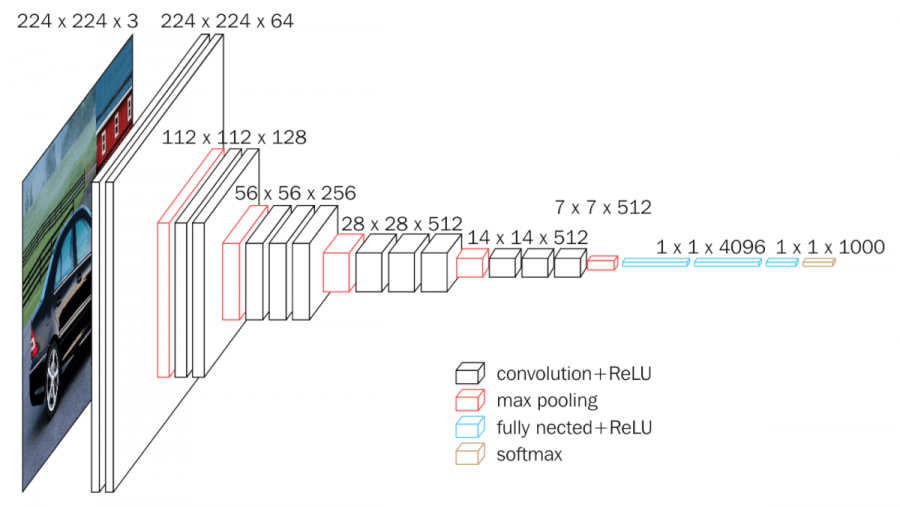
\includegraphics[width=1\textwidth]{Figures/vgg19.png}
\captionsetup{font=small}
\vspace{10pt}
\caption{VGGNet architecture.}
\label{fig:unet}
\end{figure}

\subsection{ResNet50}
\begin{figure}[!hbtp]
\centering
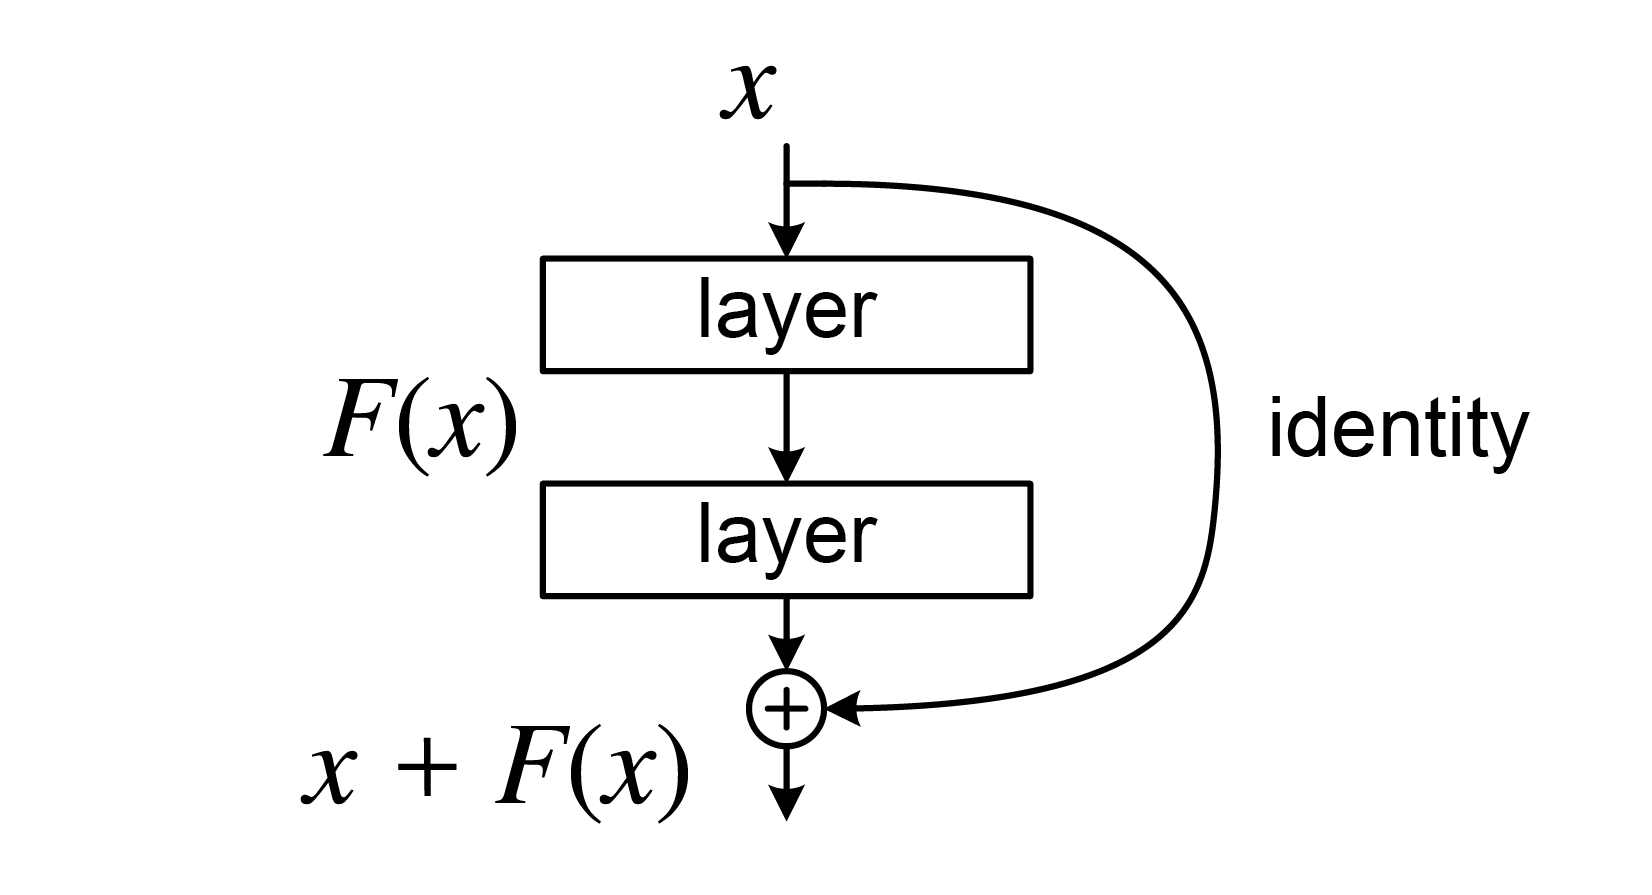
\includegraphics[width=0.6\textwidth]{Figures/ResBlock.png}
\captionsetup{font=small}
\caption{A building block of Residual Learning.}
\label{fig:resnet}
\end{figure}
ResNet-50 is a convolutional neural network with 50 layers.It is trained on more than a million images from the ImageNet database and can be used as pre-trained model with encoder decoder architecture. Here, in each residual block
the output is added with initial input through skip connection which is called the main principle of the residual network. So, it can address the vanishing gradient problem and minimize it.

\subsection{DenseNet169}
DenseNet-169 \cite{huang2018densely} is a convolutional neural network (CNN) architecture with 169 layers deep. The DenseNet architecture is known for its dense connectivity pattern, where each layer is connected to every other layer in a feedforward fashion. Here in dense block,it consists with multiple convolution layers and also no downsampling occured after each convolution. So the feature maps remain same size after each convolution which will be concatenated with next feature map. Here the concatenation is occured by using skip connections. Because each layer of the dense block is connected with other convolution layers by the skip connection. 
Besides in tansition layer,it consists with convolution and pooling layers and pooling reduces feature map sizes to reduce parameters to reach the bottleneck . This allows the network to learn both low-level and high-level features in a single pass and helps to combat the vanishing gradient problem. The dense connectivity and feature reuse in DenseNet create a more direct and efficient path for information and gradients to flow through the network during both forward and backward passes. This helps to alleviate the vanishing gradient problem.
\begin{figure}[!hbtp]
\centering
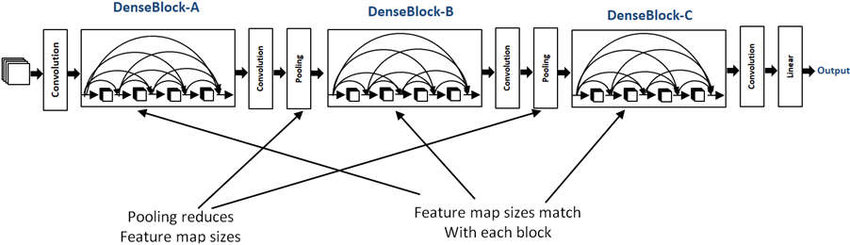
\includegraphics[width=1\textwidth]{Figures/The-architecture-of-DenseNet-121.png}
\captionsetup{font=small}
\vspace{5pt}
\caption{Densenet architecture with three dense blocks.}
\label{fig:resnet}
\end{figure}
\subsection{Inception Resnet V2}
Inception-ResNet-v2 \cite{szegedy2016inceptionv4}, a convolutional neural network, was trained with more than a million images from the ImageNet database. The network, which has 164 layers, can identify images of objects into 1000 different categories. As a result, the network has trained an enormous variety of feature representations that are rich in images. The input image has a resolution of 299 by 299 pixels, and the network produces a list of estimated class probabilities as its output.
By incorporating residual connections, the Inception-ResNet-v2 convolutional neural architecture builds upon the Inception family of architectures.
\\\\In the architecture of Inception resnet V2, there are three types of inception blocks which are Inception Resnet Block A, Inception Resnet Block B, Inception Resnet Block C, two types of Reduction Block A and B, Stem Block and Average Pooling layer. Using dropout with keeping value 0.8 to reduce the overfitting issue. Here the Inception Blocks are occured multiple times to form a full layer architecture.\\
\begin{figure}[!hbtp]
\centering
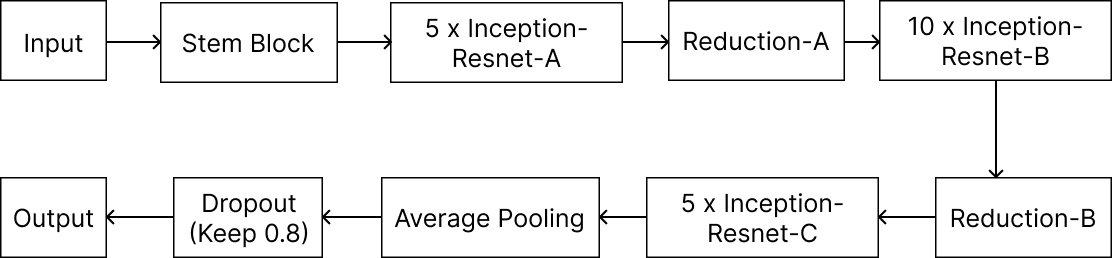
\includegraphics[width=1\textwidth]{Figures/irv2_arc.png}
\captionsetup{font=small}
\vspace{10pt}
\caption{The basic architecture of Inception Resnet V2.}
\label{fig:resnet}
\end{figure}

\begin{figure}[!hbtp]
\centering
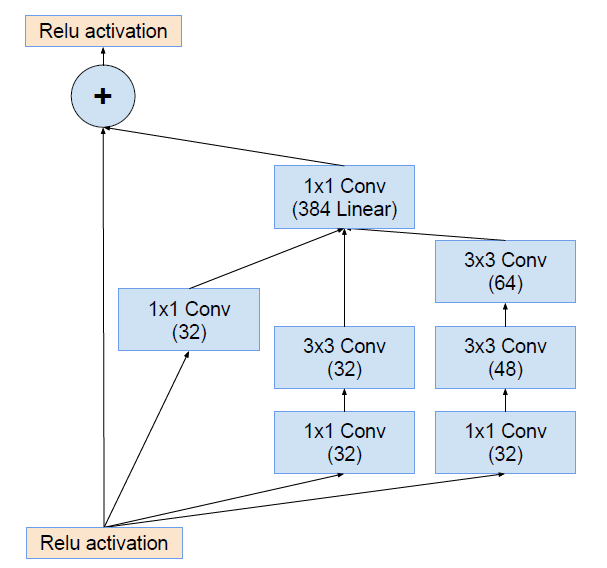
\includegraphics[width=0.6\textwidth]{Figures/inception_resnet_A.png}
\captionsetup{font=small}
\caption{Block architectue of Inception Resnet A.}
\label{fig:resnet}
\end{figure}
Inception Resnet A is one of the fundamental components of the Inception-ResNet v2 architecture. The goal of this block is to efficiently capture multi-scale properties in order to solve the vanishing gradient problem.
The Initial-ResNet-A block usually consists of the following components:\\
\textbf{Branches with Various Convolutional Kernels:}
Generally a block consists of many branches, each of which employs different kernel sizes (1x1, 3x3, 5x5) for convolutional layers. The network can thus record characteristics at different spatial scales.Here 1x1 Conv filter is used before one 3x3 Conv filter to limit the number of parameters and 5x5 filter is factorized into two 3x3 Conv to reduce the number of parameters.\\
\textbf{Residual Connections:}
Here the links allow the gradient to move more quickly on both forward and backward trips across the network. They help mitigate the vanishing gradient problem, which makes it easier to train very deep networks.\\
\textbf{Batch Normalization and Activation:}
To stabilize and activate the features, batch normalization and activation functions, typically ReLUs—are carried out after each convolutional process.\\
The general organizational structure of the Inception-ResNet A block can be seen of as an assembly of parallel branches with convolutional layers patterned after Inception and residual connections modeled after ResNet.

\begin{figure}[!hbtp]
\centering
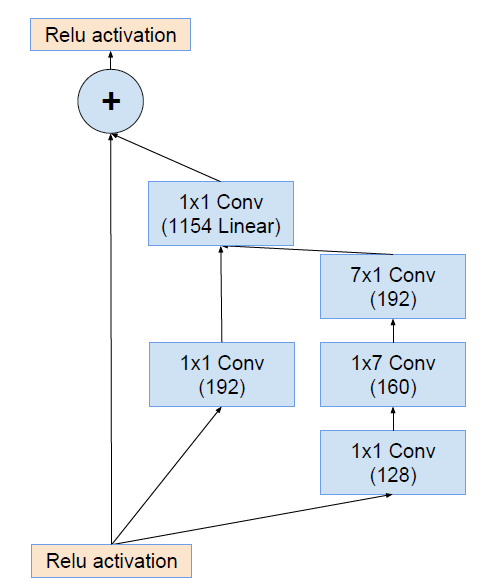
\includegraphics[width=0.6\textwidth]{Figures/inception_resnet_B.png}
\captionsetup{font=small}
\caption{Block architectue of Inception Resnet B.}
\label{fig:resnet}
\end{figure}
Another convolution block consist with 7x7 convolution filter where this filter is factorized into  1x7 and 7x1 two assymetric convolutions. This basically reduced the number of parameters.Here the 1x1 Conv is used before 7x7 Conv to limit the number of parameters as well.\\\\
Inception Resnet C is the another inception block in Inception Resnet V2 architecture where 3x3 convolution filter is used and before it 1x1 Conv is also used to reduce the parameters.Here, 3x3 convolution is also factorized into two asymmetric convolutions.The convolutions are occured parallelly and finally, all the outputs are concatenated. In this architecture, five times the Inception-Resnet-A block, ten times Inception-Resnet-B block and also five times of Inception-Resnet-C block are used with corresponding reduction blocks A and B.
Reduction blocks are mostly used to reduce the spatial dimensions of feature maps prior to feeding them into higher layers. This leads to a reduction in computational complexity, allowing the network to focus on capturing more abstract and higher-level data. Additionally, the receptive field is increased and a larger context is captured by the model by reducing the spatial dimensions.

\begin{figure}[!hbtp]
\centering
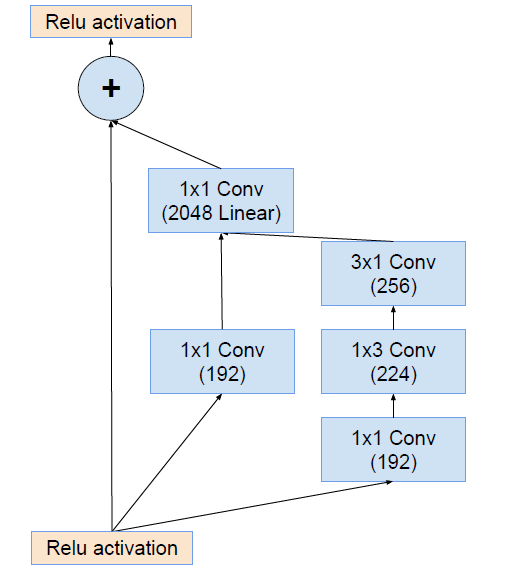
\includegraphics[width=0.6\textwidth]{Figures/inception_resnet_C.png}
\captionsetup{font=small}
\caption{Block architectue of Inception Resnet C.}
\label{fig:resnet}
\end{figure}

\begin{figure}[!hbtp]
\centering
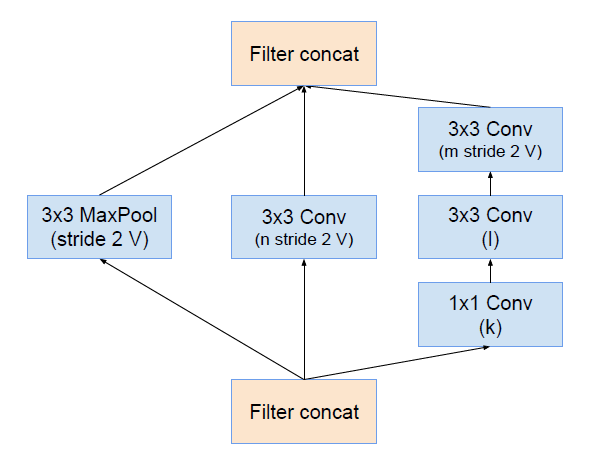
\includegraphics[width=0.7\textwidth]{Figures/reduction_A.png}
\captionsetup{font=small}
\caption{Block architectue of Reduction A.}
\label{fig:redA}
\end{figure}
\newpage
In Inception-ResNet-V2 architecture, the term "reduction block" refers to the part of the network where spatial dimensions are reduced and as a result the parameters are also reduced. This reduction is achieved by using convolutional layers with a stride greater than 1 or by using pooling operations. In IRv2 architecture there are two types of reduction blocks which are Reduction block A and B and they play a crucial role in reducing the spatial dimensions of the feature maps while preserving important information. Reducing spatial dimensions is beneficial for several reasons, including computational efficiency and the creation of a more compact feature representation.
In Figure 1.8, it deontes the Reduction A block which contains convolutional 
layers with stride, pooling operation, dimensionality reduction and shortcut connection. Here the stride is 2 and k, l, m, n denotes the filter bank where the filter bank is the collection of multiple filters arranged systematically. The value of k, l, m, n are respectively 256, 256, 384 and 384 for the Inception-Resnet V2.\\\\
Again the Reduction-B block is specifically designed to reduce the spatial dimensions of feature maps while increasing the number of channels. Similar to other blocks in the Inception-ResNet-V2 network, Reduction-B block plays a great role in down-sampling the feature maps to capture high-level features as well as feature maps efficiently. The architecture of Reduction-B block is given below.\\

\begin{figure}[!hbtp]
\centering
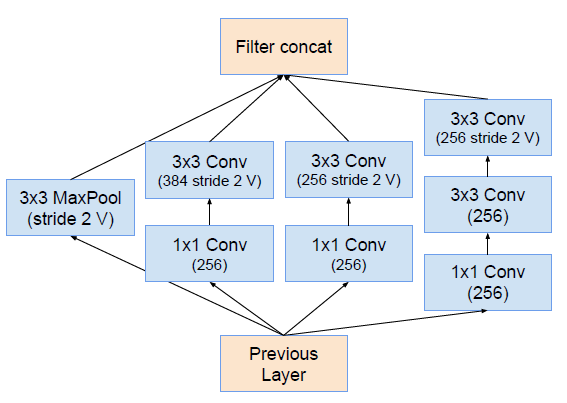
\includegraphics[width=0.7\textwidth]{Figures/reduction_B.png}
\captionsetup{font=small}
\caption{Block architectue of Reduction B.}
\label{fig:redA}
\end{figure}
\newpage

\begin{figure}[!hbtp]
\centering
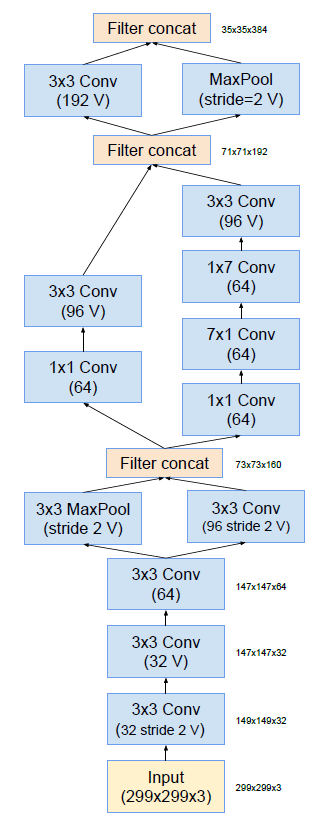
\includegraphics[width=0.5\textwidth]{Figures/stem_block.png}
\captionsetup{font=small}
\vspace{5pt}
\caption{Block architecture of the stem.}
\label{fig:redA}
\end{figure}

The above figure denotes the stem block of Inception-Resnet V2 architecture where the block is used at the vary first time to extract the initial feature of the image.
\newpage

\subsection{Datasets}
There are some labeled datasets which consist with RGB images with their corresponding ground truth depth maps that are used to train and evaluate the model.Some most used datasets for the purpose are NYU-Depth V2 \cite{laina2016deeper}, KITTI \cite{kitti}, DIODE \cite{diode}, Make3D etc.In this model, NYU-Depth V2 \cite{laina2016deeper}  dataset is used which consists with labeling and has three types of data.Those are train, test and validation data.\\
\textbf{Train data:}
The machine learning algorithm is developed using this kind of data. The input data that corresponds to an expected outcome is fed into the algorithm by the data scientist. The model continuously assesses the data to gain a deeper understanding of the data's behavior, after which it modifies itself to fulfill its intended function.\\
\textbf{Validation data:}
During training, the model is supplied new data that it hasn't evaluated before. Using validation data, which provides the initial test against unknown data, data scientists can evaluate how well the model predicts based on the new data. While some data scientists do not use validation data, it can provide insightful information for refining hyperparameters, which impact the model's data evaluation process.\\
\textbf{Test data:}
Once the model is built, testing data verifies that it can generate accurate predictions. The testing data shouldn't have labels if the training and validation data utilize labels to track the model's performance metrics. In order to confirm that the machine learning algorithm was effectively trained, test data provides the most comprehensive practical validation of an unknown dataset.

The structure of NYU-Depth V2 dataset:
\begin{itemize}
    \item 1449 pairs of RGB and depth image alignment with densely labels.
    \item 464 scenes which are new and captured from three cities.
    \item 407,024 new unlabeled frames
    \item Every item has a lebel and an instance number assigned to it. The dataset consists of several components.
    \item Labeled: A segment of the video that exhibits a high level of label density across multiple classes. Preprocessing was also applied to this data to fill in any gaps in the depth labels.
   \item Raw: The Kinect's unfiltered RGB, depth, and accelerometer data.
   \item Toolbox: Useful utilities to handle data and labels.
\end{itemize}


\subsection{Others}
There are some other tools which are used to implement the depth estimation model are likely to be loss functions with tuning, evaluation matrix, fine tuning of other pre-trained models etc.


\section{Unfamiliarity of the Problem}
There are some of the key areas where the problem can be particularly unfamiliar and challenging. Lack of accurate ground truth depth map, lack of efficient model architecture considering lower expensiveness and accuracy,  ambiguity, data quantity and quality, model complexity etc are mostly common.
There are some existing approaches to implement depth estimation model where increasing accuracy is the main factor.Various kinds of datasets ,models and other tools are used to implement it.If the image is too much noisy then proper depth map generation may be failed. So using more deeper network with different filtering approach in convolution layer may be effective to increase the accuracy and using lower number of parameters may reduce the model complexity.
So using pre-trained model with annotated dataset, helps to generate the depth map of the complex objects with higher resolution as well.

\section{Project Planning}
A well-structured project plan increases the likelihood of project success, facilitates project management, and optimizes resource allocation. It is essential to update and adjust the plan frequently to ensure that it remains aligned with the project's evolving needs and circumstances. Therefore, the planning phase is crucial to the success of any project.\\\\
From Feb 21, 2023 to Feb 15, 2024 is the whole and estimated project completion time.
Here from Feb 21, 2023, it takes 21 days to research and select the thesis topic. Then to learn about depth knowledge about the the topic it takes almost 28 days which is the literature review time. After around one month try to improve to existing work which are already done on the topic. Then from July 19,2023 experiment was started. After that
within October the basic implementation of the experiment was done. After that some different strategies and methods are applied on the implementation for the improvement and compared them with other one. Then, the result analysis was started to fix the bugs and make the work more improved efficiently. Though there were some issues to implement it like low processing speed and takes more time to execute makes it more slower. After starting the experiment, writing a report was started on the topic and it was continued till January, 2024.
Here report is written with specified formate which was given with required contents. Till now the progression of the work in provided in the chart.And finally, almost all the implementation is done with a good improvements of the existing model within Feb 15, 2024. Besides it is the plan to spent more time about result analysis to optimize the works. Here is the Gantt chart of the planning.
\subsection{Gantt Chart}
A Gantt chart is a visual representation of a project schedule that shows the timeline of various tasks or activities along with their dependencies. It provides a graphical view of the project plan, allowing project managers and team members to understand the schedule, track progress, and manage resources effectively.
The Gantt Chart for project planning is shown in \autoref{fig:gantt}.
% \begin{figure}[!hbtp]
% \centering
% 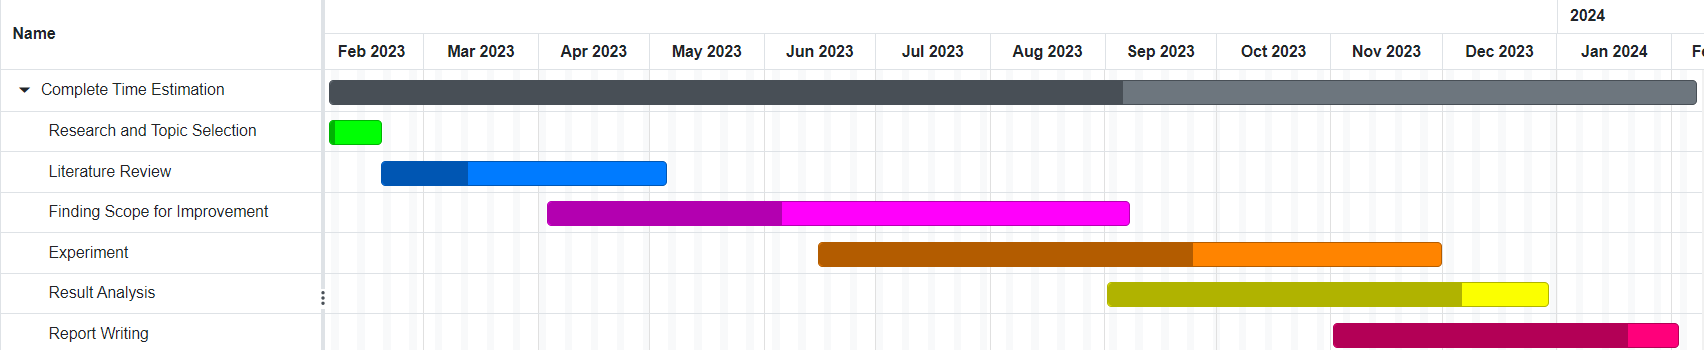
\includegraphics[width=15.5cm,height=5.7cm]{ganttchart.png}
% \captionsetup{font=small}
% \caption{Gantt-Chart for Project Planning.}
% \label{fig:gantt}
% \end{figure}

\begin{figure}[htbp]
  \centering
  \resizebox{\linewidth}{!},
        group label font=\bfseries\fontsize{50}{60}\selectfont,
        milestone label font=\bfseries\fontsize{50}{60}\selectfont,
        chart/.append style={
          canvas/.style={fill=gray},
        },
        bar/.append style={
          fill=white, % Change to black!100 for completely black
        },
        bar incomplete/.append style={
          fill=black!70, % Change to the desired color for the unfilled part
        },
       canvas/.style={ % Background color of the entire chart
          fill=gray!60,
        },
      ]{2023-02-01}{2024-2-29}
  
      \gantttitlecalendar{year, month=shortname} \\
  
      \ganttbar[progress=50, bar progress label font=\bfseries\fontsize{30}{40}\selectfont, bar progress label anchor=west, bar progress label node/.append style={right=5pt}]{Topic Selection}{2023-02-3}{2023-02-21} \\
      \ganttbar[progress=30, bar progress label font=\bfseries\fontsize{30}{40}\selectfont, bar progress label anchor=west, bar progress label node/.append style={right=5pt}]{Literature Review}{2023-03-01}{2023-05-30} \\
      \ganttbar[progress=80, bar progress label font=\bfseries\fontsize{30}{40}\selectfont, bar progress label anchor=west, bar progress label node/.append style={right=5pt}]{Finding Scope}{2023-06-15}{2023-08-10} \\
      \ganttbar[progress=20, bar progress label font=\bfseries\fontsize{30}{40}\selectfont, bar progress label anchor=west, bar progress label node/.append style={right=5pt}]{Experiment}{2023-08-01}{2023-10-20} \\
      \ganttbar[progress=80, bar progress label font=\bfseries\fontsize{30}{40}\selectfont, bar progress label anchor=west, bar progress label node/.append style={right=5pt}]{Result Analysis}{2023-11-10}{2023-12-30} \\
      \ganttbar[progress=50, bar progress label font=\bfseries\fontsize{30}{40}\selectfont, bar progress label anchor=west, bar progress label node/.append style={right=5pt}]{Report Writing}{2023-08-10}{2024-2-20} \\
      
      % You can add more tasks here
      
    \end{ganttchart}
  }
  \captionsetup{font=small}
  \vspace{5pt}
  \caption{Gantt Chart for project planning.}
  \label{fig:gantt}
\end{figure}
\newpage

\section{Applications of the Work}
i. Autonomus Driving\\
ii. Augmented Reality\\
iii. Navigation Systems and Tracking\\
iv. 3D Reconstruction\\
v. Medical Imaging and Robotics\\
vi. Automatic 2D-to-3D conversion in film\\
vii. Shadow mapping in 3D computer graphics\\
viii. Scene comprehension and simultaneous localization and mapping (SLAM)
\section{Organization of the Thesis}
The thesis is organized with all the steps to implement monocular depth estimation with other related topics.
The report started with title page.There is an acknowledgement section. List of tables and figures are identified individually in this report. The report is divided into five chapters. In \autoref{chap:intro}, basic introduction with background, objectives, scopes and project planning with gantt chart are discussed.
In \autoref{chap:lit_review}, there are some literature reviews included. The most and pupular literatures are reviewed here about monocular depth estimation and the literatures which are beneficial to understand the topic with different terms are analyzed properly. Here, the accuracy of different approaches and their effectiveness are compared. Besides, the basic functionalities which are needed to implement a model and their effectiveness are also highlighted in this section. After that some research gap solutions are identified in this chapter.
In \autoref{chap:method}, the methodology with necessary figures with equations are highlighted clearly. Here the working principle and the procedure about depth estimation models are analyzed. The model implementation associated with different functions and other models are analyzed here. After analyzing some models, the execution steps is focused here which can provide better improvements than before.\\\\
The implementation and the results are discussed in \autoref{chap:results_disc}. Here the objectives which are achieved till now are provided. The results which are basically a predicted depth map are shown with different images serially by comparing with the corresponding depth map and RGB images from the test dataset. Here the comparison is occured among different pretrained models by the percentage of mean accuracy and loss value helping with customized loss and accuracy functions. The depth map is shown using inferno-r cmap function for good visualization.  In \autoref{chap:social} by analyzing intellectual, ethical, safety and legal considerations the imapact of the thesis on societal, health and cultural issues are discussed here.
\\\\
Moreover, there are some complex engineering problems and activities which are associated with current thesis are highlighted in this \autoref{chap:prb and act}. Such as sensor modality where the choice of sensor has a big impact on the depth estimate. Different sensors, such as RGB-D cameras, LiDAR, ToF, stereo, and monocular cameras, have different features and challenges. And data collection where the quality and diversity of the dataset are significant factors. Putting together annotated data with accurate ground truth depth information can be a laborious task. Ensure that the collection include a range of environments, lighting conditions, and object types. 
And finally in \autoref{chap:concl}, the overall summary of the thesis are described in a paragraph where different kinds of model architectures with their impacts, advantages and disadvantages and other essential functions are described. Besides the challenges and limitations which are already faced are highlighted and the future works of our project are also discussed in this chapter.

%%%%%%%%%%%%%%%%%%%%%%%%%%%%%%%%% Literature Review %%%%%%%%%%%%%%%%%%%%%%%
\chapter{\textbf{Literature Review}}\label{chap:lit_review}
\section{Introduction}This literature review aims to critically evaluate and summarize previous research, shedding light on important themes, approaches, and conclusions pertaining to monocular depth estimation. The objective in reviewing the literature is to find gaps, inconsistencies, and new patterns that will guide future research efforts.
The literatures which are related to monocular depth estimation are reviewed here.
%  (\autoref{chap:lit_review}) explains the related literature ...
% \autoref{chap:method} ...

\section{Literature Review}
% Cite papers as necessary \citep{hasan2020investigation,yaganoglu2021real}. \citet{bird2020optimisation} proposed ...
An improved model to present a convolutional neural network for computing a high-resolution depth map given a single RGB image with the help of transfer learning \cite{c1}. Here the depth map
captured object boundaries more faithfully with fewer parameters and less training iterations.In this paper, in preprocessing steps the image is flipped horizontally if required which is called image augmentation. Besides tuning of the loss function by changing with weights make it more perfect. A straightforward encoder-decoder architecture with skip connections is used here where the
encoder part is used as a pre-trained truncated DenseNet-169 \cite{articledense} .In quantitavely the method may not be best but the quality of the produced depth map is much better. Here the accuracy on the test dataset (NYU-Depth V2) is 84.6\% which is better than other previous results and using other pretrained model with fine tuning can make it more accurate.
\\\\
Another proposal is a fully convolutional architecture, encompassing residual learning, to model the ambiguous mapping between monocular images and depth maps \cite{c2}.It also focused on the improvement of 
the output resolution through efficient learning of feature map upsampling.The model is trained end-to-end
and does not contains any post processing techniques like CRFs or other refinement techniques.The proposed architecture builds upon ResNet-50.Here NYU Depth v2 dataset is used where the size of
the input image is 302x228. Here the error rate is 0.573 in RSE and 0.195 in RMSE(log) which are better than other approaches.
\\\\
An approach \cite{c3} of using the tools that enable mixing multiple datasets during training, even if their annotations are incompatible.Basically,  the experiments confirm that mixing data from complementary sources greatly improves monocular
depth estimation.Mixing multiple datasets like NYU Depth v2, KITTI, TUM, DIODE etc. provides better accuracy than individual one.
\\\\
A method \cite{c4} to match detailed depth boundaries without the need for superpixelation.A 
regress on the depth using a neural network with two components happened here. one that first estimates the global
structure of the scene, then a second that refines it using local information. The network is trained
using a loss that explicitly accounts for depth relations between pixel locations, in addition to pointwise error. The system achieves state-of-the art estimation rates on NYU Depth and KITTI, as well
as improved qualitative outputs.Here the RMSE(linear) error is 7.156 and the RMSE(log) error is 0.270 as well.
\\\\
A double estimation method \cite{c5} that improves the whole-image depth estimation and a patch selection method that adds local details to the final result.Here using modified MiDaS network ,the RMSE error is 
0.1598.The method is demonstrated by merging estimations at different resolutions with changing context to generate high resolution depth map.
\\\\
With a good benchmark values,one of the methods is GAN based monocular depth estimation \cite{c6} which works with three processes.Those are segmentation and depth estimation, adversarial loss calculations
and cycle consistency loss calculations.NYU Depth v2 data set is here with the RMSE of 0.652 and RMSE(log) is 0.217 approximately.
\\\\
In inception-Resnet V2 \cite{szegedy2016inceptionv4}, training with residual
connections accelerates the training of Inception networks significantly. It consists with 164 layers and worked on ImageNet dataset. In the architecture of the Inception-Resnet V2, there are three Inception-Resnet block and two reduction block. The inception blocks are used repeatedly at the time of training. In each block, there are 1x1, 3x3 and 5x5 types of convolution filters. Here the 1x1 Conv block is used before other filters to limit the number of parameters and asymmetric factorization on these filters plays a great role to reduce the number of parameters. Different sizes of these filters make it more versatile to extract the different sized features from an image. In this architecture, the input image size is 299x299 which can be RGB image.In this paper, different kinds of Inception architectures are analyzed. Such as, Inception V1 (GoogleNet), Inception V2, Inception V3, Inception V4, Inception-Resnet V1 and Inception-Resnet V2. Basically, the literature showed about the improvement of the inception architecture using Residual network.\\\\
A less complex Convolutional Neural Network (CNN) architecture is used to predict coarse depth, and surface normal guidance is then used to improve the coarse depth pictures.
Compared to the current states, more comprehensive depth maps are generated with fewer network parameters and a more straightforward learning framework. Uisng less parameters makes it more faster for execution with considering detailed depth map. Furthermore, the framework's suitability for integration into a monocular simultaneous localization and mapping (SLAM) paradigm is confirmed by 3D point cloud maps that are rebuilt from depth prediction pictures.
In this paper \cite{article_sf}, the contribution is reflected in proposing an RGB-D surface normal network, which eectively captures the geometric relationships between RGB and depth images. Here the performance is evaluated on NYU-Depth V2 dataset and the RMSE error is 0.459 with 18 epochs. Besides by using Densenet 121 with 32.4 M parameters, the accuracy is 0.859 (85.9\%) for the test set of the dataset.The subject of future study is pre-trained depth estimation networks which will be used to 3D vision techniques like SLAM, SFM, and AR (simultaneous localization and mapping). 
\section{Discussion of Research Gap Solution }
To generate depth map using depth estimation, there are many more gaps and challanges which are needed to be solved. Analyze the complexity of the models is one of the major concerns. Another key points are edge handling and scale ambiguity which can be handled by evaluating depth maps. Besides there is a enough lack of accuracy of the generated depth map compared to ground truth depth map. So using fine tuning of the pre-trained model can put a great contribution to improve the accuracy.
Identifying research gaps is a crucial aspect which has some potential solutions like multi-model fusion, some post-processing techniques, data synthesis, hybrid architectures, loss function configuration etc. Now the table proves that the problem idea is a new one and not acquired directly from existing sources.


\begin{table}[!htb]
\centering
\begin{threeparttable}
\captionsetup{font=small}
\caption{Table for proving the thesis idea unique.}
\label{tab:test}
\small % Reduce font size

\begin{tabular}{|p{0.25\linewidth}|p{0.35\linewidth}|p{0.30\linewidth}|}
\hline
\multicolumn{1}{|c|}{\textbf{Proposed Method}} & \multicolumn{1}{c|}{\textbf{Research Gap}} & \multicolumn{1}{c|}{\textbf{Solution}} \\  
\hline
High Quality Monocular Depth Estimation via Transfer Learning \cite{c1}
results high quality depth map with good resolution. &
Fine tuning of the more efficient pre-trained model with less number of parameters can improve the depth map visualization  &
The model can be more flexible using lower number of parameters.So using U-Net architecture with Inception-Resnet V2 \cite{szegedy2016inceptionv4} as an encoder can be effective. \\ \hline

Another proposal is a fully convolutional architecture, encompassing residual learning, to model the ambiguous mapping between monocular images and depth maps \cite{c2}. &
The model is trained end-to-end
and does not contains any post processing techniques like CRFs or other refinement techniques.Here, the error rate is 0.573 in RSE while using NYU Depth V2 dataset. &
Using post processing technique is one of the vital tasks to make the depth estimation model more accurate.The proposed model can hopefully reduce this error. \\ \hline

Towards Robust Monocular Depth Estimation: Mixing Datasets for Zero-shot Cross-dataset Transfer &
The model can not find the depth map of the printing or painting image it occured in the basis of reflections of the pixels. &
Our model hopefully estimate the depth map for the printing image as well as the noisy image using preprocessing of the model. \\ 
\hline

A double estimation method \cite{c5} that improves the whole-image depth estimation. &
Here using modified MiDaS network ,the RMSE error is 
0.1598 and needs high resolution image to train the model. &
Using high resolution image datasets can be huge and needed higher end pc to be executed.So using low resolution image with deeper network can increase accuracy. \\ 
\hline

With a good benchmark values,one of the methods is GAN based monocular depth estimation \cite{c6} &
NYU Depth v2 data set is here with the RMSE of 0.652 and RMSE(log) is 0.217 approximately. &
The accuracy can be improved with reducing the error rate by tuning loss functions. \\ 
\hline

A method \cite{c4} to match detailed depth boundaries without the need for superpixelation. &
The method can not improve quantitative output that means there can be high errors. &
Considering these, the improvement method is concerned about both qualitative and quantitative errors and increase the accuracy to find complex object's depth map. \\ \hline
\end{tabular}

\end{threeparttable}
\end{table}


% \begin{center}

% \end{center}

%%%%%%%%%%%%%%%%%%%%%%%%%%%%%%%%% Methodology %%%%%%%%%%%%%%%%%%%%%%%
\chapter{\textbf{Methodology}}\label{chap:method}

\section{Introduction}
This section describes the encoder-decoder architecture that is used to estimate a depth map from a single RGB image. Next, the relationship between the complexity of the encoder and decoder and performance is examined. The next suggestion is a suitable loss function for the task at hand. Lastly, effective augmentation policies are given that greatly facilitate the training process.
\section{Proposed Methodology}
\subsection{Problem Design and Analysis}
Using U-Net architecture with normal encoder-decoder will not be able to generate better depth map. But the model can be fine tuned using pretrained model provides better accurate result. So neet to implement a model via transfer learning with proper optimization algorithm. So, to make a proper model, it is necessary to follow the organized way for implementing the model. At the below sections, all the steps are provided sequentially.
\subsection{Data Collection and Preprocessing}\label{sec:sec_1}
This is the initial steps to collect dataset from online resources or real life resources. Then preprocess the dataset to resize every elements of it and make it convenient to implement with models.Besides, normalization and augmentation are more effective in pre-processing.\\\\
Selecting dataset is the main concern on which the execution or run time and the accuracy of the model depends on.Here NYU-Depth V2 \cite{laina2016deeper} dataset is used which is basically an indoor dataset consisting with both RGB images and GT depth map where the data is divided into three sets: training, testing, and validation sets. In this dataset the image size is 640x480 with containing 120k training samples and 654 testing samples. But the model is trained on 65k subset. At the time of preprocessing, the images are resized into same sizes which are used as input. Then normalization is occured within [0 to 1]. After that, horizontal flipping (i.e. mirroring) of images are considered at a probability of 0.5.
Ground truth depth map is used to find the accuracy by comparing with estimated depth map and also used to train the model as depth estimation model.
\subsection{Model Architecture}
Secondly , a CNN based simplified depth estimation model is selected which follows U-Net architecture. The model is implemented with the help of tensorflow python framework or library. The U-Net is an encoder-decoder network, with the RGB image as input and depth map as output.The encoder network
consists of convolution and pooling layers to capture the depth features, and the decoder network includes deconvolution layers to
regress the estimated pixel-level depth map, with the same size as the input.In encoding and decoding section, upsampling and downsampling are occured respectively.\\\\
In this thesis, U-Net architecure is used to implement the model, but at the encoder part of the architecture, it is substituted by some high performing pre-trained models. So, here the down-sampling is occured via truncated pre-trained model's layers and at the decoder section, the previous downsampled images are concatenated with upsamplemd images by skip connections. Therefore, as pretrained models, Resnet50, Densenet169, VGG19 and Inception-Resnet V2 \cite{szegedy2016inceptionv4} are used and among them using Inception-Resnet V2 provides a better result as an encoder. The Inception-Resnet V2 has three inception block with consisting of different sizes of convolution filters. And each block can be repeated multiple times in the architecture. Here, the model is trained using 15 epochs on the train set because more than 15 epochs causes overfit issue. In each epoch, the forwardpass is occured among the layers and resulted the predicted values. After that the predicted values are compared with actual values and loss values are found using appropriate loss functions.
This is called finding gradient and then descent the loss, the backwardpass is occured and then previous weights are updated by new weights.
So, in this model 'Adam' gradient-discent optimization algorithm is used. It is known as adaptive moment estimation. This is the method which can compute adaptive learning rate for each parameters.
% \subsection{A Subsection Under the Section}
% You can place necessary equation, such as \autoref{eqn:test}.
% \begin{equation}
% 	F_i''=\lvert F_i-2F_{i-1}+F_{i-2} \rvert 
% 	\label{eqn:test}
% \end{equation}

% where, $i$ ...

% \subsection{Another Subsection Under the Section}

% The logo of KUET is shown in \autoref{fig:unet}.
\newpage
\begin{figure}[!hbtp]
\centering
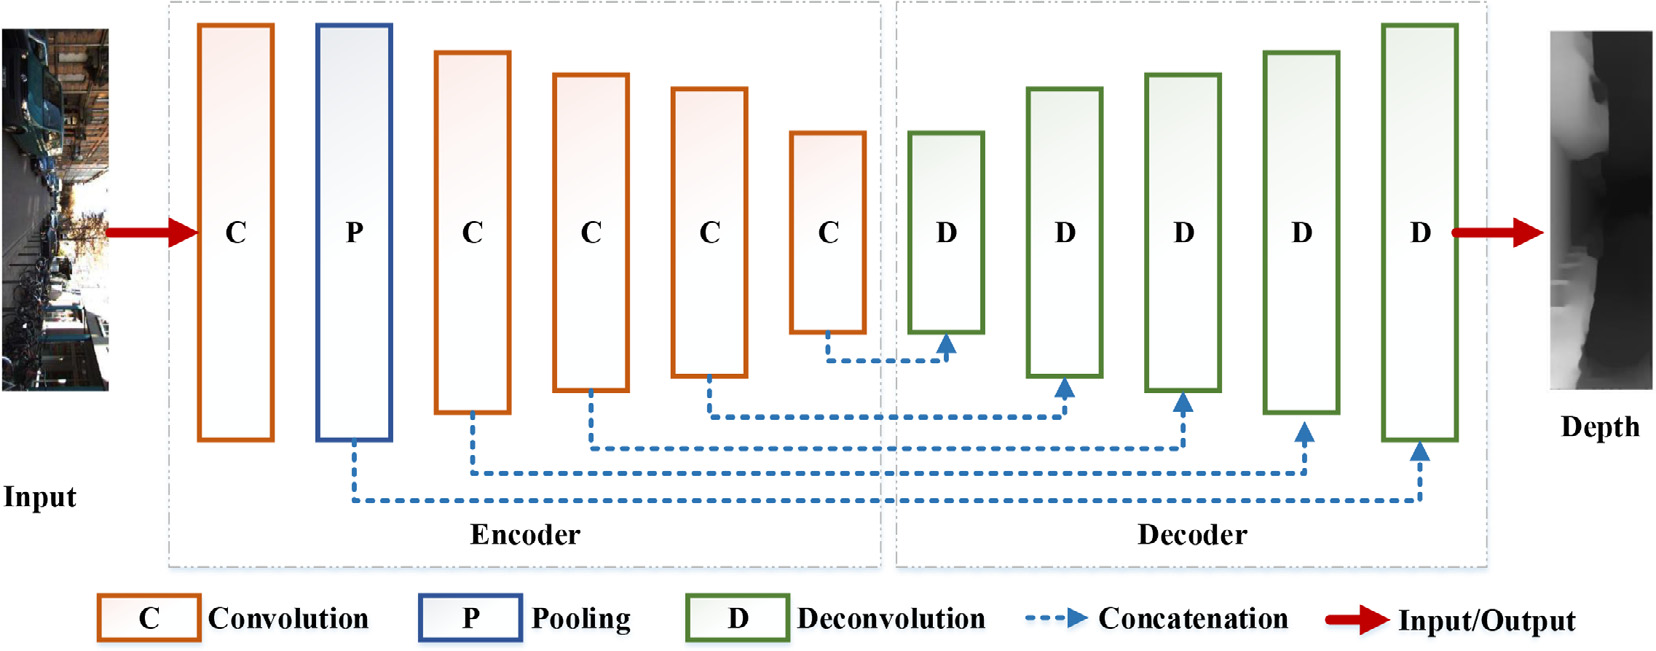
\includegraphics[width=1\textwidth]{unet.png}
\captionsetup{font=small}
\caption{The CNN based general pipeline of deep learning for monocular depth estimation.}
\label{fig:unet}
\end{figure}
\\\\
The above figure defines the fully connected convolutional network which is consisted with both convolutional and pooling layer in encoding poriton where through downscaling the image resolution is also reduced. In decoding section,additive skip-connections are implemented in the downscaling block where the deconvolution and unpooling are occured to recover the image with higher resolution.This is basically an U-Net architectural model which is used to segment to object to generate the depth map. As it is an encoder-decoder network, the encoder can part can be used as other pre-trained layers of the model which makes great contribution of the result. Using the network, the overall depth estimation model structure is given below.
\\\\

\begin{figure}[!hbtp]
\centering
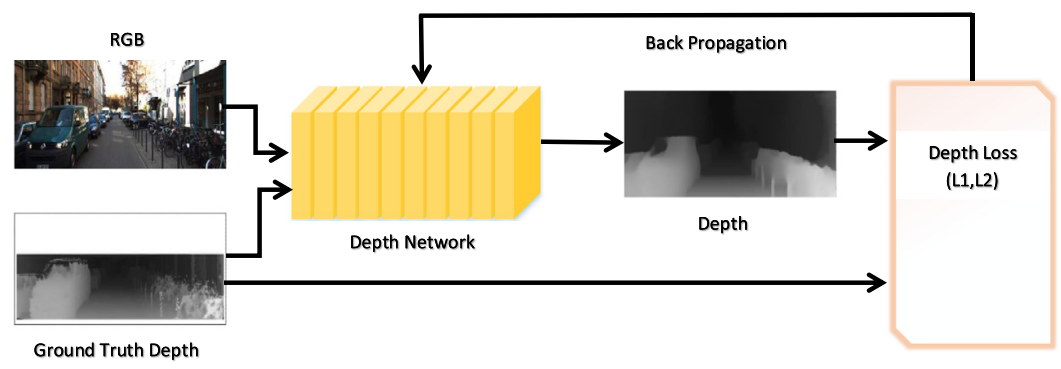
\includegraphics[width=1\textwidth]{model.png}
\captionsetup{font=small}
\vspace{5pt}
\caption{The general model of supervised learning for monocular depth estimation.}
\label{fig:model}
\end{figure}
\newpage
\begin{figure}[!hbtp]
\centering
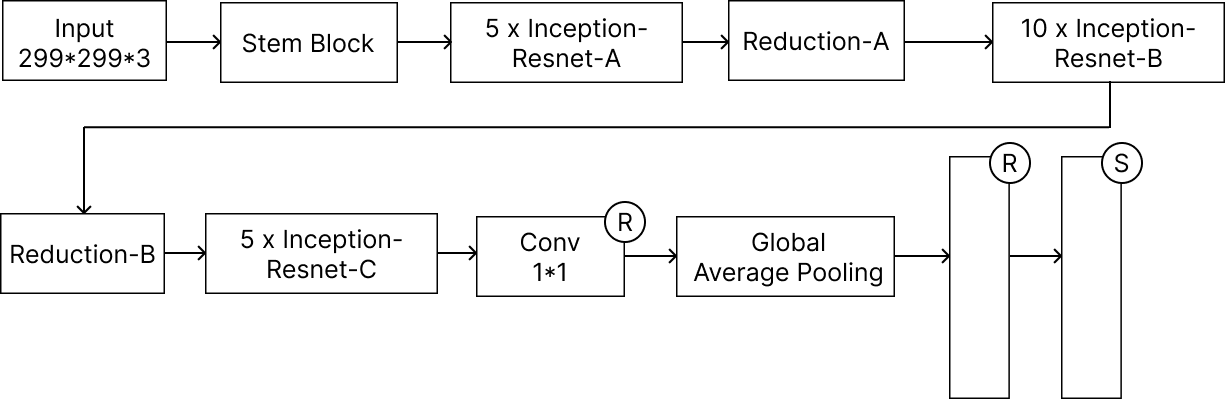
\includegraphics[width=1\textwidth]{Figures/Irv2_workflow.png}
\captionsetup{font=small}
\vspace{10pt}
\caption{The flow diagram of Inception-Resnet V2. }
\label{fig:model}
\end{figure}

\vspace{2cm}

\begin{figure}[!hbtp]
\centering
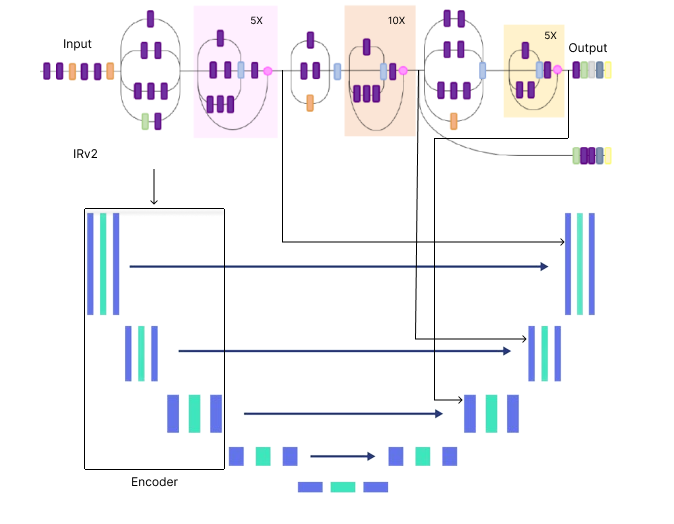
\includegraphics[width=1\textwidth]{Figures/full_model_2.png}
\captionsetup{font=small}
\vspace{2pt}
\caption{The detailed architecture of U-Net with Inception-Resnet V2.}
\label{fig:model}
\end{figure}

\newpage
In the final model, it is built on U-Net architecure with the help of high performing Inception-Resnet V2 pretrained model which help to generate more detailed and high quality depth map with better accuracy than other models. Here, the truncated layers of IRv2 are used for the purpose of downsampling and then the image is decoded with simplified way.


\subsection{Building a Data Pipeline}
The pipeline takes a dataframe containing the path for the RGB images, as well as the depth and depth mask files.
It reads and resize the RGB images.
It reads the depth and depth mask files, process them to generate the depth map image and resize it.
It returns the RGB images and the depth map images for a batch.
\subsection{Building the model}
For building the model, there are two important functions need to implement. One is downsampling the block in encoder section and the other one is upsampling the block in the decoder section where skip-connections are implemented in the downsampling block. Here, the truncated layers of IRv2 are used for downsampling through convolution and pooling and then the downsampled image is concatenated at the time of upsampling through skip connection. Basically at bottleneck, a bridge establish the connection  between encoder and decoder for upsampling and recovering the depth map.

\subsection{Loss Function}
The difference between the groundtruth depth map $y$ and the predicted depth map $\hat{y}$ is taken into account by a typical loss function for depth regression issues. The training pace and total depth estimation performance can be greatly impacted by various loss function factors. A wide range of loss function modifications are used to optimize the neural network for depth estimation. In this report a customize loss funnction is used which helps to improve the accuracy of the model by tuning weight.
For training the network, loss L is defined between
$y$ and $\hat{y}$ as the weighted sum of three loss functions:

\begin{equation}
    L(y, \hat{y}) = \lambda L_{\text{depth}}(y, \hat{y}) + L_{\text{grad}}(y, \hat{y}) + L_{\text{SSIM}}(y, \hat{y})
\end{equation}

where $L_{\text{depth}}$, $L_{\text{grad}}$, and $L_{\text{SSIM}}$ are depth, gradient, and SSIM loss terms, respectively.


\begin{equation}
        L_{\text{depth}}(y, \hat{y}) = \frac{1}{n} \sum_{p}^{n} \left| y_p - \hat{y}_p \right|
        \label{eqn:eq2}
\end{equation}
\begin{equation}
        L_{\text{grad}}(y, \hat{y}) = \frac{1}{n} \sum_{p}^{n} \left| g_x(y_p , \hat{y}_p) \right| + \left| g_y(y_p , \hat{y}_p) \right|
        \label{eqn:eq2}
\end{equation}
\begin{equation}
        L_{\text{SSIM}}(y, \hat{y}) = \frac{1 - \text{SSIM}_(y, \hat{y})}{2}
        \label{eqn:eq2}
\end{equation}

Here, $L_{\text{depth}}$ is the point-wise L1 loss defined
on the depth values, $L_{\text{grad}}$ is the L1 loss defined over
the image gradient g of the depth image and $L_{\text{SSIM}}$ uses the Structural Similarity (SSIM) term which is a commonly-used metric for image reconstruction
tasks.

\section{Conclusion}
In conclusion, the proposed methodology represents a depth estimation model which can generate depth map with high detailing of the image. Here the methedology is described by analyzing all the steps which are needed to make the model. Besides the full model architecture is highlighted here with better visualization to make the better understanding of it. In this model, the customized loss function is described in more precisely where the functions can be tuned using several weights.

% \section{Loss Function}
% A loss function is used during the training phase of a deep learning model.
% It provides a measure of the error between the predicted values and the true(GT) values, and the goal during training is to minimize this error.There are common equations to calculate the errors are:
% \\
% \begin{equation}
%         \mathit{RMSE} = \sqrt{\frac{1}{N} \sum_{i=1}^{N} (y_i - \hat{y}_i)^2}
%         \label{eqn:eq2}
% \end{equation}
% \begin{equation}
%     \log(\mathit{RMSE}) = \left(\sqrt{\frac{1}{N} \sum_{i=1}^{N} (\log(y_i) - \log(\hat{y}_i))^2}\right)
%     \label{eqn:eq2}
% \end{equation}
% \begin{equation}
%     \text{ARE} = \frac{1}{N} \sum_{i=1}^{N} \left| \frac{y_i - \hat{y}_i}{y_i} \right|
%     \label{eqn:eq3}
% \end{equation}

% \begin{equation}
%     \text{SRE} = \frac{1}{N} \sum_{i=1}^{N} \left \frac{(y_i - \hat{y}_i)^2}{y_i} \right
%     \label{eqn:eq4}
% \end{equation}
% \section{Post-processing}
% Post processing is an important task for refine the output generated by training model.It is actually use to get more detailed depth map with higher resolution and high amount of edge detailed.
% \section{Visualizing Model Output}
% After generating the estimated depth map, it must be necessary to monitor the estimated depth map before performing improvementing tasks and it should be occured repeatedly until reaching the goal.
% \section{Possible Improvement}
% Here, the major improvement is to increase the accuracy and reduce the error of the predicted depth map compared with GT depth map.To increase the accuracy there are two cases. One is to make the more deeper network that means add extra layer with existing layer and the other case is generate the depth map for noisy image where the existing model may fail but the proposed method with different filtering approach provide better result with good accuracy than existing methods.
% \section{Result Analysis}
% It is the analyzing steps to identify the strength of the model.Before and after improvement, it must be necessary to check the accuracy or the error rate.Evaluation matrix is used to analyze the result with helping of both quantitative and qualitative evaluation.
% \\\\Generally,Lower error rate means good result as well as higher accuracy and according to the error rate, the improvement will be continued.If the desired accuracy is achieved, then the objectives will be full-filled.

%%%%%%%%%%%%%%%%%%%%%%%%%%%%%%%%%%%%%%%%%%%%%%%%%%%%%%%
\chapter{\textbf{Implementation, Results and Discussions}} \label{chap:results_disc}

\section{Introduction}
In the implementation phase, the proposed methods are applied sequentially to implement the final model in order to get the desired depth map with better detailing of the objects. Here, the implementation of the model is described and after that, the predicted results are analyzed with depth map visualization and finally, compare the depth map with ground trupth depth map by considering different pre-trained models. Evaluation martrics are used in this section for the comparison through finding the loss values and accuracy values after training of the model.

\section{Experimental Setup}
The optimal setup proposed by the author is divided into two parts. One is hardware setup and the other one is software setup.\\
\textbf{Hardware Setup:}
\begin{itemize}
  \item Camera: A monocular camera can capture RGB image.
  \item Sensor: At the time of capturing the image,it can measure the depth between two objects. Such as Lidar which can calculate the depth more precisely.
  \item Computer: GPU which can accelarate the training of the model and so NVIDIA GPUs are commonly used to train.
  \item Storage: The dataset which is larger, needs the memory to store it and besides, in the storage the trained model is saved.
  \item Power Supply: Ensuring of a stable power supply is necessary.
\end{itemize}
\newpage
\textbf{Software Setup:}
\begin{itemize}
  \item Operating System: Choose a operating system which is compatible with Linux, Windows and Mac OS.
  \item Deep Learning Frameworks: To implement the model, Keras is used where Keras is a high level API of tensorflow framework.
  \item Depth Estimation Model: U-Net architecture with IRv2 pre-trained model as an encoder.
  \item Libraries and Dependencies: Various kinds of libraries and dependencies are used which are already integrated in Keras. Such as OpenCV, Numpy, Matplotlib etc.
  \item Evaluation tools: For the evalution of the result, the error metrics are used for qualitative evaluation.
  \item Dataset: NYU-Depth V2 dataset, which is appropriate for depth estimation model is also used to train the model.
\end{itemize}

\section{Evaluation Metrics}
The error metrics which are defined for the evaluation of the model are defined by the following equation which is called quantitative evaluation.
\\
\begin{equation}
        \mathit{RMSE} = \sqrt{\frac{1}{N} \sum_{i=1}^{N} (y_i - \hat{y}_i)^2}
        \label{eqn:eq2}
\end{equation}
\begin{equation}
    \log(\mathit{RMSE}) = \left(\sqrt{\frac{1}{N} \sum_{i=1}^{N} (\log(y_i) - \log(\hat{y}_i))^2}\right)
    \label{eqn:eq2}
\end{equation}
\begin{equation}
    \text{ARE} = \frac{1}{N} \sum_{i=1}^{N} \left| \frac{y_i - \hat{y}_i}{y_i} \right|
    \label{eqn:eq3}
\end{equation}

\begin{equation}
    \text{SRE} = \frac{1}{N} \sum_{i=1}^{N} \left \frac{(y_i - \hat{y}_i)^2}{y_i} \right
    \label{eqn:eq4}
\end{equation}

\section{Dataset}

This study uses the 640 x 480 resolution NYU Depth v2 dataset, which provides photos and depth maps for a variety of interior settings. A training subset of 65K samples is used with the dataset, which has 120K training samples and 654 testing samples. Ten meters is the top limit on the depth maps. The network produces predictions with a resolution of 320 x 240, which is half of the input resolution. The input photos are downscaled to 320 x 240 while the ground truth depths are maintained at their original resolution for training purposes. In the testing stage, the whole test image's depth map prediction is calculated and then upsampled by two times to match the resolution of the ground truth. 

\section{Implementation and Result}
In this phase, after completing the initialization and preprocessing steps the built model is executed for the training on NYU-Depth V2 dataset where the image is already preprocessed. It takes 15 epochs to train the model which provides the best result rather than more than 15 epochs. For the epoch, gradient discent optimization algorithm is used 
named 'Adam'. Besides the loss function is customized here which can tune the loss values in order to find the best weights. Evaluation matrics are implemented to compare and evaluate the model with other models and determines it's accuracy.

\begin{figure}[!hbtp]
\centering
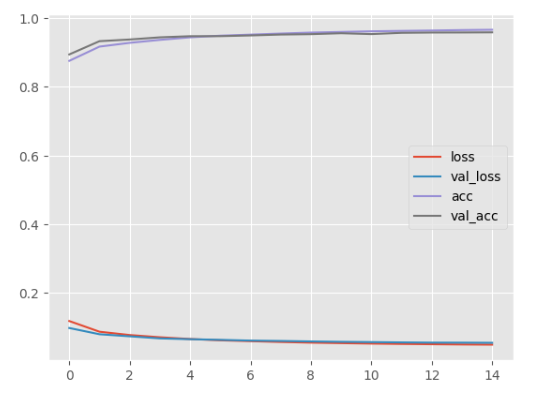
\includegraphics[width=.7\textwidth]{Figures/accuracy_graph.png}
\captionsetup{font=small}
\caption{Loss and accuracy graph of training and validation set of the model.}
\label{fig:ind}
\end{figure}
The above graph determines the loss and accuracy of the train and validation set of the dataset. Here the above two curves denote the train and validation accuracy and the below two curves determine the train and validation loss. It is cleared that, initially there is a quite bit difference between train and validation loss as well as accuracy. But after some epochs, the training accuracy is getting closer to the validation accuracy. i.e the more closer training curve to validation curve, the more accurate the result is. So we got the highest accuracy is 0.8533 and the lowest loss is 0.1523 after fitting the model.\\\\
The depth maps which are generated using the trained models are given below. Here, the original image, their corresponding  ground truth depth map and the predicted depth maps are provided in a row consecutively.
Besides the detailed depth maps are visualized using inferno-r color map which is basically represented by RGB image and lower the intensity of the pixel means, higher the distance of the object from the camera.\\

\begin{figure}[!hbtp]
\centering
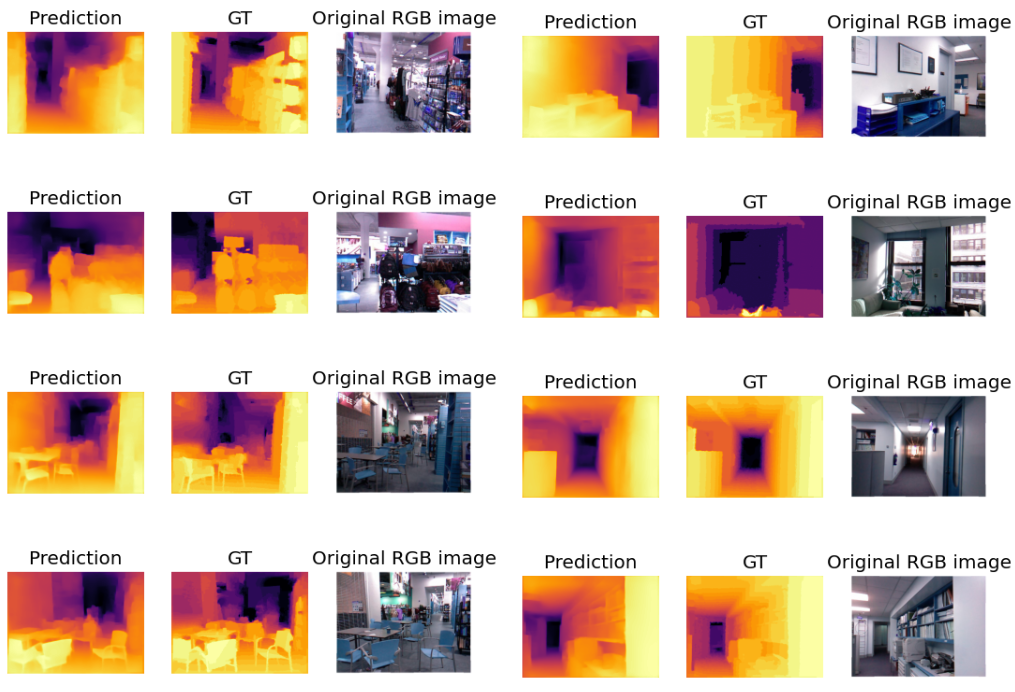
\includegraphics[width=1\textwidth]{Figures/result.png}
\captionsetup{font=small}
\caption{Generated depth maps with their corresponding ground truth depth maps of the RGB images.}
\label{fig:out}
\end{figure}
% You can tabulate your result like \autoref{tab:test}.
\newpage

\begin{table}
  \centering
  \caption{Evaluation metrics with different types of models.}
  \begin{tabular}{lcccccc}
    \toprule
    \textbf{Model Name} & \textbf{Parm.} & \textbf{Epochs} & \textbf{RMSE} $\downarrow$ & \textbf{ARE} $\downarrow$ & \textbf{CLFE} $\downarrow$ & \textbf{Accuracy} $\uparrow$ \\
    \midrule
    Enc-Unet & 8.6 M & 15 & 0.0063 & 0.0238 & 0.1921 & 0.7642 \\
    Resnet50 & 14.4 M & 15 & 0.0069 & \textbf{0.0149} & 0.1675 & 0.8073 \\
    VGG19 & 22.4 M & 15 & 0.0098 & 0.0559 & 0.1711 & 0.7979 \\
    Densenet169 & 12.2 M & 15 & \textbf{0.0057} & 0.0406 & 0.1538 & 0.8489 \\
    IRv2 & 31.1 M & 15 & 0.0066 & 0.0710 & \textbf{0.1524} & \textbf{0.8533} \\
    \bottomrule
  \end{tabular}
  
  \label{tab:evaluation}
\end{table}
In this table, CLFE stands for Error by Customized Loss Function. RMSE is Root Mean Squared Error and ARE is called as Absolute Relative Error. Besides, the Inception Resnet V2 model is defined as IRv2. After analyzing the evaluation metrics, using IRv2 model can provide higher accuracy on test data of NYU-Depth V2 dataset. But in overall cosideration, Densene169 has almost closer accuracy to IRv2 but it has huge lower parameters and so densenet169 is more convenient in this case. Here, lower the value of RMSE, ARE, CLFE and higher the value of the accuracy denotes good result.\\\\
\textbf{Quantitative results.} Here the amount of RMSE error for IRv2 model is lowest, CLFE is also lower than others, but ARE error is lower in the resnet50 model. So by using overall considerations, IRv2 can be better model to improve the result. \textbf{Qualitative results.} Here the customized loss function is used to evaluate the quality of the model on NYU-Depth V2 dataset. Here, three types of loss functions are used to find the tuned values in field of depth estimation. One loss is point wise loss, another one is gradient loss and finally SSIM loss is calculated and the merging of these three losses build a well tuned function to define the quality. U-Net with normal encoder-decoder provides the accuracy of 0.7642 but using IRv2 as an encoder with U-Net improves the accuracy drastically which is 0.8533.

\section{Objective Achieved}
Almost all the objectives which are planned from started are achieved. The plan was using different types of high-performing pretrained model as an encoder can improve the accuray and so using IRv2 is able to improve the accuracy rather than using the Densenet169. Though there are still some issues about train time, but that is not the concern here where accuracy is the main focused.

% \section{Morality or Ethical Issues}
% Generating depth maps using monocular depth estimation techniques can raise several morality and ethical concerns, as they intersect with various aspects of technology, privacy, and societal impact.\\\\
% Generating depth maps using monocular depth estimation techniques can raise several morality and ethical concerns, as they intersect with various aspects of technology, privacy, and societal impact.Besides,depth estimation algorithms might not always provide accurate depth maps, and errors could lead to incorrect conclusions or judgments.It has some great impacts because of it's application fields like autonomus driving,medical imaging,robotics etc.
% Just like any technology, depth maps can be misused for malicious purposes.It is so much cost effective and time consuming to built and run the depth estimation model.


% \section{Socio-Economic Impact and Sustainability}
% Monocular depth estimation in deep learning are multifaceted and extended across various domains.Monocular depth estimation, as a component of computer vision, can lead to the development of innovative products and services, spurring economic growth and job creation in sectors such as augmented reality, robotics, autonomous vehicles and many more.Depth estimation plays a great role in the field of medical imaging used to find tumor cells from human organs. Efficient use of depth estimation in applications like autonomous vehicles can lead to optimized navigation which has a great impact on society. Besides, the adoption of monocular depth estimation and related technologies necessitates a skilled workforce, leading to opportunities for education and skill development in AI, computer vision, and related fields.

% \subsection{The Impact of the Project on Societal, Health, Safety, Legal and Cultural Issues}
% ......
% \subsection{The Impact of Project on the Environment and Sustainability}
% .......
\section{Financial Analysis and Budget }
Financial analysis and budget in monocular depth estimation is complex because it depends on various factors including the scope of the project, resources required, team size, infrastructure costs and more. But there are some requirements which are needed to implements and advertise the depth estimation model and those are equipment or software, dataset, publication fees etc. Here it was tried to minimize the financial cost by using online IDE like kaggle where it provides the facilities of GPU. Besides it provides a larger storage to save the model and store the dataset. Moreover, in this IDE it supports all kinds of python framework like tensorflow which makes it more easier to implement the model. So, these kinds of facilities reduce the financial cost drastically. Using table, it can be analyzed considering general factors and basic requirements. Besides the total budget allocation for maintaining the thesis is given through table.
\\
\begin{table}[!htb]
\centering
\begin{threeparttable}
\captionsetup{font=small}
\caption{Table for Financial Budget Plan.}
\label{tab:test}
\small % Reduce font size

\begin{tabular}{|p{0.40\linewidth}|p{0.28\linewidth}|}
\hline
\multicolumn{1}{|c|}{\textbf{Budget Category}} & \multicolumn{1}{c|}{\textbf{Estimated Cost}} \\  
\hline
Software and Equipment & 500-1000 BDT\\ \hline
Cost for Dataset & 200-500 BDT\\ \hline
Cloud Computing Service & 1000-1500 BDT \\ \hline
Infrastructure & 800-1000 BDT \\ \hline
Miscellaneous & 500-1000 BDT \\ \hline
Total Estimation of Budget & 3000-5000 BDT \\ \hline
\end{tabular}

\end{threeparttable}
\end{table}

\vline
\begin{table}[!htb]
\centering
\begin{threeparttable}
\captionsetup{font=small}
\caption{Table for Financial Analysis.}
\label{tab:test}
\small % Reduce font size

\begin{tabular}{|p{0.40\linewidth}|p{0.50\linewidth}|}
\hline
\multicolumn{1}{|c|}{\textbf{Field}} & \multicolumn{1}{c|}{\textbf{Analysis}} \\  
\hline
Research and Development & Licensing fees for using existing deep learning frameworks or libraries\\ \hline
Infrastructure and Computing Resources & Cost of hardware and software for developing and testing the depth estimation models \\ \hline
Validation and Testing & Resources needed for testing the accuracy and costs associated with creating validation datasets \\ \hline
Project Management & Compensation for project managers and coordinators \\ \hline
Marketing and Communication & Budget for promoting the project's outcomes \\ \hline
Sustainability and Long-Term Costs & Cost for maintaining and updating the models and software \\ \hline
\end{tabular}

\end{threeparttable}
\end{table}

\section{Conclusion}
In conclusion, there are some basic implementation which must be needed to run the model properly. After implementing the model, the required output was found with a good accuracy but not the best. Here, the accuracy and the loss are measures through evaluation functions which are also discussed in this section. But to do all these things, financial analysis with the budget plan is required which provides the overall estimated cost to conduct the thesis. Though this is not the best way to improve the accuracy but, the idea leads to another better path for the same purposes.
In summary, even if the current implementation shows encouraging results, more study and development are needed to address current issues and advance the field of depth estimation. Beyond theoretical frameworks, the model's potential use is demonstrated by its effective implementation in autonomous navigation.



%%%%%%%%%%%%%%%%%%%%%%%%%%%%%%%%%%%%%%%%%
\chapter{\textbf{Social Health, Environment, Safety, Ethical, Legal and Cultural Issues}}\label{chap:social}
\section{Introduction}
This chapter demonstrates the socio-economic impact and the ethical, safety, and legal considerations in the field of monocular depth estimation. It also describes the intellectual properties considerations and societal, health and cultural issues in this phase.
\section{Intellectual Property Considerations}
The legal and ethical considerations surrounding the use of datasets and models have received careful consideration throughout this thesis. A thorough approach to securing the necessary consents and authorizations from the relevant creators or owners of the datasets and models is combined with strict adherence to ethical norms. To ensure the highest regard for intellectual property rights and adherence to usage terms, a rigorous mechanism is in place. Additionally, a concentrated effort is made to provide credit and recognition to the original writers, both as a demonstration of intellectual integrity and as a way to foster a courteous and cooperative academic atmosphere. By upholding these principles, this thesis ensures the responsible and ethical use of data, honors the rights of content creators, and advances transparency in the realm of research practices.
\section{Ethical Considerations}
There are several ethical concerns with the use of depth estimation model. Concerns are raised by the advanced estimation technology's ability to measure distance with high resolution. Given that depth estimation model have the capacity to produce harmful effects—such as harmful robot design for wrong purposes. it is crucial that moral guidelines and standards be established in order to prevent any improper use of this technology. In doing the thesis, caution was taken to ensure that no privacy was violated by the data used to train the model. Furthermore, it is now crucial to establish moral standards for usage.
\section{Safety Considerations}
The thesis is established based on the model which needs to be trained on a large dataset, and originality of the dataset was a concern throughout the whole process.  Before the training of the model, the data had been preprocessed and  after training post processing refines the output but it had been made sure of the fact that, no original information carried in the data or image does not get altered in the process. This ensures the security of the depth estimation model. Because if the data in the object is altered, then there is a huge possibility of generating a significant error which can be more dangerous in the fields of it's applications. It only generates the depth map, keeping the original details of the image intact.
\section{Legal Considerations}
The thesis centers its legal concerns on three main issues: intellectual property, copyright, and responsibility. The dataset that was used for training and testing was, first of all, freely available to the public and contained no copyrighted content. It is essential to acknowledge that no private or personal data was included in the study without express consent from the relevant owners.
Furthermore, there are possible hazards associated with developing any depth estimate methodology, especially when using it. As users are ultimately accountable for the pictures that the model processes, an application monitoring mechanism must be in place. This methodology guarantees an anticipatory response to any unanticipated difficulties or moral dilemmas that can emerge when applying the depth estimation model.
\section{Impact of the Project of Societal, Health and Cultural Issues}
The thesis on depth estimation has important ramifications for several social, health, and cultural concerns, which might lead to both opportunities and difficulties:\\\\
\textbf{Social Impact:}
Depth estimation facilitates the making of apps for virtual reality (VR) and augmented reality (AR), advertising immersive communication experiences in a variety of social scenarios. Concerns about privacy violation are raised by the broad use of depth estimating systems. Strong privacy frameworks must be established in order to protect people's personal information and stop unlawful data gathering as these technologies become more widely used.\\\\
\textbf{Health Impact:}
Medical imaging applications rely heavily on depth estimation algorithms to help with details diagnosis and treatment planning of a wide range of medical disorders. It helps with the accurate measuring of tumor forms, sizes and locations in oncology.
With the use of technology, telemedicine solutions may be developed, giving medical personnel the ability to evaluate patients' illnesses from a distance and deliver prompt interventions, especially in underserved or rural places.\\\\
\textbf{Cultural Impact:}
Depth estimation uses 3D scanning and modeling techniques to help preserve cultural heritage places and items. It makes it possible to create digital duplicates of historical sites and objects, ensuring their preservation and availability for the next generations.
Through the creation of immersive experiences and virtual exhibits, it expands the creative possibilities in the entertainment and art sectors.


\section{Impact of the Project on the Environment and Sustainability}
The environmental and sustainable effects of a depth estimate project might take many different forms, with both positive and negative outcomes.\\\\
\textbf{Positive Impacts:}
\begin{itemize}
\item An essential component of robotics and autonomous systems is depth estimation. Improved depth sensing can result in autonomous navigation that is more energy-efficient, which makes lower total energy consumption in applications including environmental monitoring, agricultural, and warehouse automation.

\item A more economical use of resources like water, fertilizer, and pesticides is made possible by precision farming, which is maintained by depth estimation in the field of agriculture. As a result, waste and environmental effects are reduced, which supports sustainable agriculture practices.

\item The depth estimate abilities of the proposed thesis may be used as the basis of application to monitor the environment, supporting activities such as tracking species, mapping habitats, and evaluation of the effects of climate change.
\end{itemize}


\textbf{Negative Impacts:}
\begin{itemize}
\item The inadequate management of electronic trash (e-waste) may result from the manufacture of depth-sensing devices like cameras and sensors. To reduce the influence on the environment, it is essential to provide appropriate recycling and eliminating procedures.

\item Large computational resources could be needed to develop reliable monocular depth estimation techniques. It is possible to reduce the possible environmental effect of algorithmic complexity by investigating optimization approaches and confirming energy-efficient implementations.

\item The resources needed to manufacture depth sensing equipment are extracted from the environment, such as metals and rare earth minerals. Initiatives for recycling and sustainable sourcing can help in addressing these issues and difficulties.

\item A major challenge is promoting sustainable applicatoins. Here, enhancing the technology's beneficial effects on the environment may be achieved by promoting the development and use of monocular depth estimation in fields like precision agriculture and environmental monitoring, which have obvious sustainability advantages.


\end{itemize}

\section{Conclusion}
In conclusion, the comprehensive evaluation of the project's social, health, environmental, safety, ethical, legal, and cultural components highlights the project's importance within the larger societal framework. The initiative emphasizes the necessity for a sensitive and responsible approach by acknowledging the interactions between technology and the several disciplines. By using these factors, the project may be made to achieve both technological and social goals, allowing innovation to be smoothly and properly incorporated into many areas of human existence. So, the thesis has a great impact on the wide range of fields, each with unique issues and outcomes.



%%%%%%%%%%%%%%%%%%%%%%%%%%%%%%%%%%%%%%%%%
\chapter{\textbf{Addressing Complex Engineering Problems and Activities}}\label{chap:prb and act}
\section{Complex engineering problems associated with the current thesis}
% In monocular depth estimation, there are several technical difficulties. Here are a few possible difficulties related to this subject:\\\\
% \textbf{Limited Data for Training:}
% In monocular depth estimation algorithms, the large and varied datasets are frequently needed for the efficient training. Such datasets can be difficult to get and require a lot of work to curate, especially when specific ground truth depth information is included.\\
% \textbf{Ambiguity in Depth Perception:}
% The inner difficulty of handling depth ambiguity from a single 2D picture arises in monocular depth estimation. Getting rid of this uncertainty and predicting depth accurately is a major technical issue, particularly in complicated scenarios which is more challenging.\\
% \textbf{Real-time Processing Constraints:}
% Efficient techniques and optimum processing efficiency are necessary for the implementation of monocular depth estimation in real-time applications like augmented reality or robotics. It takes a good trade-off to accomplish both precision and speed. But less optimized model causes a bad impact for getting better accuracy.\\
% \textbf{Handling Dynamic Environments:}
% It is difficult to adapt monocular depth estimation methods to dynamic situations with moving objects or shifting scenery. In real-world applications, it is essential to provide stable performance in scenarios with changing circumstances.\\
% \textbf{Integration with Existing Systems:}
% Monocular depth estimation requires proper collaboration and compatibility to be integrated into current systems, such as self-driving cars or medical imaging applications. Overcoming integration obstacles is essential for successful implementation in the real life applications.\\
% \textbf{Optimizing for Edge Devices:}
% Lightweight and power-efficient depth estimation models are needed for a wide range of applications, including edge computing platforms and mobile devices. An unique engineering problem is balancing model complexity with resource limitations.\\
% \textbf{Handling Occlusions and Object Interactions:}
% It is difficult to address issues with occlusions and object interactions in a scene. The depth estimation problem becomes more complicated when it tries to estimate accurate depth maps, especially when there are overlapping objects involved in the image.\\
% \textbf{Robustness to Adverse Conditions:}
% One of the constant challenges in engineering is creating depth estimation models that works with complex circumstances like dim illumination, reflection, bad weather, or difficult textures. Improving the resilience of the model guarantees consistent performance with good detailing of the depth map in real-world scenarios.

\begin{table}[!htb]
\centering
\begin{threeparttable}
\captionsetup{font=small}
\caption{Table for complex engineering problems associated with the current thesis.}
\label{tab:test}
\small % Reduce font size

\begin{tabular}{|p{0.20\linewidth}|p{0.03\linewidth}|p{0.67\linewidth}|}
\hline
\multicolumn{1}{|c|}{\textbf{Attribute}} & {\textbf{ }} & {\textbf{Address the Attributes of Complex Engineering Problems
}} \\  
\hline
Depth of knowledge required & P1 &
In the thesis, the proper reviews are occured on deep learning and monocular depth estimation. Besides, for choosing the appropriate model, deeper knowledge is necessary to know about the strengths and weakness of the model. The thesis includes training process, hyperparameters and loss function tuning, optimization alogrithms etc which helps to increase the knowledge more deeper. And also the thesis defines and justifies the evaluation metrics and their implementations to compare the model with others.\\
\hline

Range of conflicting requirements & P2 &

There is a major confliction occured between accuracy and computational efficiency. Because it is hard to maintain high accuracy and computational efficiency at the same time. Besides a conflict occurred between data quality and quantity whether to use high resolution data is hard with a large amount. So the adjustment is occured in the thesis with using proper ways to solve these. \\ \hline

Depth of analysis required & P3 &
The depth of analysis is reflected in the following key areas with their comprehensive analysis. Those areas are literature review, model selection and architecture, dataset analysis, training strategies, evaluation metrics, ethical implications etc.
 \\ \hline


% Depth of analysis required &

% Our model hopefully estimate the depth map for the printing image as well as the noisy image using preprocessing of the model. \\ 
% \hline

Familiarity of issues & P4 &

The thesis identifies and discusses key challenges to monocular depth estimation, such as handling occlusions, addressing scale ambiguity, and dealing with limited training data. So, identifying challenges demonstrates a deep understanding of the unique issues associated with monocular depth estimation.  \\ 
\hline

 Extent of applicable codes & P5 &
 Here the attributes are considered as code implementation, code documentation, code validation and testing, code integration etc. which can ensure the applicability of the thesis fields.
 \\ \hline

 Extent of stakeholder involvement and conflicting requirements & P6 &
 The thesis begins by identifying and categorizing relevant stakeholders associated with the idea.Besides gathering feedback from them is important to resolve the conflicts.
 \\ \hline
% Extent of applicable codes &

% The accuracy can be improved with reducing the error rate by tuning loss functions. \\ 
% \hline

% Extent of stakeholder involvement and conflicting requirements
%  &

% Considering these,our improvement method is concerned about both qualitative and quantitative errors and increase the accuracy to find complex object's depth map. \\ \hline

Interdependence & P7 & 
Interdependencies occurred  between the choices of hyperparameters and model performance. Good initialization of the hyperparameters make the model more appropriate. The justification is that, the thesis addresses the interdependence between the model's performance and its adaptability to diverse real-world scenarios. \\ \hline
\end{tabular}

\end{threeparttable}
\end{table}

\newpage
\section{Complex engineering activities associated with the current thesis}
% 
\begin{table}[!htb]
\centering
\begin{threeparttable}
\captionsetup{font=small}
\caption{Table for complex engineering activities associated with the current thesis.}
\label{tab:test}
\small % Reduce font size

\begin{tabular}{|p{0.22\linewidth}|p{0.03\linewidth}|p{0.65\linewidth}|}
\hline
\multicolumn{1}{|c|}{\textbf{Attribute}} & {\textbf{ }} & {\textbf{Address the Attributes of Complex Engineering Activities
}} \\  
\hline
Range of resources & A1 &
In this thesis, the computational resources are needed to train and implement deep learning models for monocular depth estimation. And the justification is, by considering computational resources, the thesis acknowledges the importance of scalability and efficiency in model development. Besides, the range of data resources needed for training deep learning models is addressed here and a variety of data resources enhances the model's ability which helps to apply in real-world applications. Hardware resources are another crucial things which should be addressed. The availability of GPUs or TPUs have a great impact on the execution of deep learning model which increases the speed and efficiency of training deep learning models. So by ensuring  hardware resources, the thesis ensures that the proposed solution is adaptable to different computing infrastructures.\\ \hline

Level of interaction & A2 &

The thesis describes the iterative process of the model, highlights the level of interaction involved in adjusting parameters, architecture, or training strategies based on feedback and intermediate results. Here the process ensures that the model evolves and improves over time. User feedback is a good thing for the interaction and so by adding user feedback, the depth estimation model becomes more applicable and relevant. Collaborative development is another level of interaction where it can lead to diverse perspectives and expertise and enrich the research.
 \\ \hline

Innovation & A3 &
 The thesis explore a innovation strategy which makes the model more prefarable to improve the accuracy. Using the Inception-Resnet-v2 pretrained model as an encoder with U-Net architecture to predict the depth map is a new thing that can provide a better result than other models. \\ 
\hline

Consequences for society and the environment & A4 &

Consequences lie in its application fields for society and the environment. Using the basic knowledge of the thesis, it may have a great impact on the field of autonomous driving, medical imaging, robotics, and other real-world applications.  \\ 
\hline

Familiarity & A5 &
The thesis shows a deep understanding of core concepts related to monocular depth estimation, including stereo vision principles, depth perception etc. which are more familiar with previous ideas described in the literature review. Familiarity with core concepts is crucial for the better implementations with innovations. Moreover, familiarity with different models is an important term in implementation. Such as IRv2 pre-trained model added extra benefits by improving the result. \\ 
 \hline
\end{tabular}

\end{threeparttable}
\end{table}


%%%%%%%%%%%%%%%%%%%%%%%%%%%%%%%%%%%%%%%%%%%%%%%%%%%%%%%%%%%%%%%%%%%%%%%%%%%%%
\chapter{\textbf{Conclusions}}\label{chap:concl}
\section{Summary}
The report introduces a convolutional neural network (CNN) for high-resolution monocular depth estimation from single RGB images, emphasizing the use of transfer learning. The network follows an encoder-decoder architecture called U-Net. In this architecture, initializing the encoder to extract features from pre-trained networks and employing augmentation, tuning of loss function and training strategies for improving accuracy. Here some pretrained networks are used like Resnet50, VGG19, Densenet169 and Inception-Resnet v2 (IRv2) and among them IRv2 provides the highest accuracy inspite of having high expensiveness. Before using a pre-trained model instead of an encoder, the U-Net (only) provides the accuracy 0.7620 but after using of IRv2 as an encoder, it produces the accuracy of 0.8533. Despite of having a simple decoder, the proposed method achieves detailed high-resolution depth maps. The network, with fewer parameters and training iterations, surpasses state-of-the-art performance on NYU-Depth v2 dataset, producing qualitatively superior results that faithfully capture object boundaries. Besides, the socio-economic impact and the ethical, safety, and legal considerations in the field of monocular depth estimation are demonstrated here and the complex engineering problems and activities are also addressed.
\section{Limitations}
The main goal is to generate a depth map with good accuracy which plays a great role in scene understanding. But there are some limitations which should be considered for the implementation:\\
i) Using larger dataset causes higher memory consumption and needed high-end pc to run the model.\\
ii) Using the truncated layers of the pre-trained model as an encoder, makes the model more complex which is computationally expensive.\\
iii) There is a higher chance to be delay issue because runtime of the model is extremely high which causes problems to train the model.\\
iv) Using a deeper network increases computational complexity as well.\\
v) If the images of the dataset are so noisy, it fails to generate a good depth map.\\
vi) The dimensions of the input image influence the number of parameters. So, using high-resolution images increases the number of parameters which can cause overfitting problems.
\section{Recommendations and Future Works}
There are some factors which should be improved to make the result more convenient. So,
there will be further testing and validations using a range of datasets and benchmarking against state-of-the-art depth estimation methods to assess the resilience and generalization capabilities of the proposed model. Besides,  fine-tuning the both trained and pre-trained model on specific target domains or datasets to enhance its performance in real-world applications. Merging multiple datasets to make it more versatile which can provide better result than before. Again optimization of the model's performance can be occured by  hyperparameter tuning, like tuning of learning rates, batch sizes, and regularization parameters. Integration of the model in the real-time application and so improve the model's ability to estimate depth in dynamic scenarios. Finally enhances the interpretability of the model, making it more transparent and understandable.\\\\
So, after considering the above recommendations, the future works are more likely to be:\\
i) Multi-model fusion to improve depth estimation accuracy and robustness.\\
ii) Fine-tuning the trained model to get a more convenient depth map.\\
iii) Continual learning approach where a model learns continuously from new data over time without forgetting the knowledge it has acquired from previous tasks. \\
iv) Using better optimization algorithm to make the model more flexible with less complexity and faster execution.\\
v) Keep the consistency of the accuracy of estimated depth map using a comparatively smaller dataset by training the model.\\
vi) Combining diverse datasets is a good strategy to enhance the model's robustness.

%\appendix
%\appendixpage
%\addappheadtotoc
%\input{"Mathematical\space definitions/draft"}

\backmatter
%\setstretch{1}
%\include{"Bibliography/draft"}
% Change title of bibliography to References
\renewcommand\bibname{References}
% Make sure "references" is in the header
% \fancyhead[RE]{\bfseries REFERENCES} % if I make it for two-sided book-like printing
% \fancyhead[R]{\bfseries REFERENCES} % if I make it for single-sided printing
% Place it in the table of contents
\newpage
\phantomsection \label{refs}
\addcontentsline{toc}{part}{References}

% Declare style
% \bibliographystyle{plainnat}
% \bibliographystyle{plain}

\printbibliography[title={REFERENCES}, notsubtype=this thesis]

% %printing publication from this thesis; entrysubtype={this thesis} is mentioned in corresponding bib file
% \nocite{hasan2021how,hasan2021effect,hasan2021tuning}
% %\newrefcontext[labelprefix=J]
% \printbibliography[title={Publications from this Thesis}, subtype=this thesis, resetnumbers=true]
% \addcontentsline{toc}{part}{Publications from this Thesis}

\end{document}
